%%%%%%%%%%%%%%%%%%%%%%%%%%%%%%%%%%%%%%%%%%%%%%%%%%%%%%%%%%%%%%%%%%%%%%%%%%%%%%%%
%\documentclass[12pt,papel,twoside]{tesis}
\documentclass[12pt,screen,twoside,pagebackref]{tesis}
%\documentclass[12pt,papel,singlespace,oneside]{tesis}
%\documentclass[12pt,papel,preprint,singlespace,oneside]{tesis}

%%%%%%%%%%%%%%%%%%%%% Paquetes extra %%%%%%%%%%%%%%%%%%%%%%%%%%%%%%%%%%%%%%%%%%%
% Por conveniencia: aqu\'{\i} puede cargar todos los paquetes y definir los comandos 
% que necesite
\usepackage{extra}
%%%%%%%%%%%%%%%%%%%%%%%%%%%%%%%%%%%%%%%%%%%%%%%%%%%%%%%%%%%%%%%%%%%%%%%%%%%%%%%%
%%%%%%%%%%%%%%%%%%%%% Informacion sobre la tesis %%%%%%%%%%%%%%%%%%%%%%%%%%%%%%%
\title{Software para medici\'{o}n de erosi\'{o}n y sedimentaci\'{o}n en modelos f\'{i}sicos por medio de relevamiento digital de superficies}
\author{Emanuel Sanchez Aimar}
\director{Mgs. Ing. Mariana Pagot}
\codirector{Dr. Oscar Bustos}
\carrera{Licenciatura en Ciencias de la Computaci\'{o}n}
\laboratorio{}
\grado{}
\palabrasclave{A definir}
\keywords{to define}
% Si queremos poner la fecha manualmente:
% \date{Diciembre de 2099}

%%%%%%%%%%%%%%%%%%%%%%%%%%%%%%%%%%%%%%%%%%%%%%%%%%%%%%%%%%%%%%%%%%%%%%%%%%%%%%%%
%\titlepagefalse % Si no quiere compilar la portada descomente esta linea
%\includeonly{apendices} % Compilar s\'{o}lo estos archivos 
\graphicspath{{figs/}} % Lugar donde encontrar las figuras generales (se puede poner uno en cada cap{\'{\i}}tulo)
%%%%%%%%%%%%%%%%%%%%%%%%%%%%%%%%%%%%%%%%%%%%%%%%%%%%%%%%%%%%%%%%%%%%%%%%%%%%%%%%


\begin{document}

% Dentro del environment 'preliminary' va:
% la dedicatoria, resumen, abstract, indices

\begin{preliminary}

% Escriba su dedicatoria
\dedicatoria{
A mi familia\\
A mis amigos\\
A todos los que me conocen\\
A toda esa otra gente que no
}

%%% \'{I}ndices %%%%
\tableofcontents                %\'{I}ndice

\begin{abreviaturas}
                                %Abreviaturas
\end{abreviaturas}

\listoffigures                  %Figuras

\listoftables                   %Tablas

\begin{resumen}

El presente trabajo plantea el desarrollo de una técnica experimental que permite medir la erosión y sedimentación en modelos físicos a escala reducida en laboratorio mediante la generación automática de un mapa 3D que representa la condición resultante de un ensayo hidráulico, utilizando una cámara RGB-D Microsoft Kinect. \\
Esta técnica se presenta ante la necesidad de realizar un relevamiento de erosión de un modo más preciso y eficiente respecto de la técnica utilizada tradicionalmente, que consiste en un relevamiento manual de puntos, generalmente haciendo uso de un nivel óptico y una mira milimétrica.\\ 
La técnica propuesta exhibe varios aspectos que superan al enfoque tradicional. En primer lugar, es una solución no intrusiva, es decir, no produce alteraciones sobre la condición del modelo. Además, mejora significativamente la resolución espacial del área medida, permite cubrir áreas extensas y disminuye el tiempo de medición de cada escenario ensayado. Los resultados obtenidos muestran que la solución propuesta permite realizar mediciones de erosión y sedimentación con una precisión superior a la técnica tradicional. \\

\end{resumen}

\end{preliminary}

% Podemos usar cualquiera de los dos comandos: \input o \include para incluir el texto
\chapter{Introducción}

\section{Motivaciones}
\label{S:motivaciones}

Los modelos fisicos hidraulicos son una de las principales herramientas que cuenta el campo de la Ingeniería Civil para la medición y estudio de la erosión, asi como la acumulacion y transporte de sedimentos.
Tradicionalmente, la medición de variables sedimentarias en laboratorio ha consistido en el relevamiento manual de puntos, generalmente distribuidos sobre una grilla equidistante, por medio de un nivel óptico y una mira.
Esta metodología, de carácter intrusiva (debido a que se apoya la mira sobre la superficie a relevar), presenta errores intrínsecos generados por la intervención humana y restricciones relativas a los instrumentos de medición, que pueden alcanzar los 1.5 cm. Algunas fuentes de error están relacionados con la incorrecta verticalidad de la mira, el apoyo del palpador sobre el modelo (que puede alterar la superficie a medir), errores en las lecturas y/o transcripción de las mismas, entre otros.

Por otro lado, la precisión de los productos derivados (curvas de nivel, modelos tridimensionales (3D), perfiles transversales, etc.) y los análisis de dichos productos, se verán afectados por la densidad de puntos relevados y la elección de los mismos.
Esta limitación produce un trade off entre la densidad de puntos obtenida, el área relevada y el tiempo dedicado a cada ensayo, que el ingeniero debe afrontar a la hora de realizar y completar un ensayo hidráulico fluvial en laboratorio. \\

%%% AGREGAR referencias

En el campo de la robótica, la construcción de mapas 3D del entorno físico ha sido considerado, por años, una tarea fundamental para su aplicación en la navegación autónoma y la manipulación de objetos por parte de un robot. Diferentes sensores han sido utilizados para lograr este propósito, entre ellos se puede mencionar el uso de sonares[ref], escáneres láser[ref], cámaras estereoscópicas[ref], cámaras RGB-D[ref], etc.
En los últimos años, sensores RGB-D como el dispositivo Microsoft Kinect han surgido en la industria del entretenimiento. Sus prestaciones técnicas y costo asequible lo han convertido en una solución idónea para ser utilizada en diferentes aplicaciones de Computer Vision, como es el caso de la generación de mapas 3D. \\

%%% AGREGAR : breve introducción en generacion de mapas 3D

En este trabajo se propone una nueva técnica para la medición de erosión en modelos a escala reducida mediante la generación automática de mapas 3D utilizando el sensor
RGB-D Microsoft Kinect. Esta técnica digital aplicada a procesos fluviales permite representar la superficie erosionada y/o sedimentada resultante de un ensayo hidráulico. \\
La metodología propuesta busca mejorar la caracterización obtenida del modelo físico debido a la mayor densidad de puntos obtenida. Además, busca relevar una mayor área y reducir el tiempo de medición. Esta técnica no es intrusiva, y se considera automática debido a que el único requerimiento del usuario es el desplazamiento de la cámara.

\section{Objetivos}
\label{S:objetivos}

El objetivo de este trabajo es desarrollar un software para la generación de un mapa 3D de un modelo físico a escala reducida utilizando una cámara RGB-D. Esta aplicación permitirá medir digital y automáticamente las variables de erosion y sedimentacion en laboratorio. \\
Para crear un mapa 3D del modelo, el sistema deberá capturar nubes de puntos del área de trabajo, alinearlas en un mismo sistema de coordenadas, filtrar posibles inconsistencias y realizar una conversión de escala modelo a prototipo. \\
Se validará esta nueva técnica digital con respecto a la técnica tradicional para realizar una evaluación de su precisión y verificar si es viable su aplicacion. \\
Dentro de este marco, se propone desarrollar una librería extensible y modular que permita la creación de nuevas aplicaciones, con el objetivo de aportar nuevas soluciones al problema de la medición de erosión. \\

%%% Local Variables: 
%%% mode: latex
%%% TeX-master: "template"
%%% End: 
\chapter{Revisión del estado del arte}
\label{cap:estado-del-arte}

En las áreas de robótica móvil y visión por computador, la construcción de mapas 3D del entorno ha sido tema de investigación por años. Diferentes sensores han sido utilizados con este objetivo, entre ellos, sensores laseres \cite{chou2013robotic,Montemerlo02fastslam}, camaras monoculares \cite{tomono2009robust,clemente_etal_rss2007}, camaras estereo \cite{Mei11,Konolige08}, entre otros. La mayoría de los sistemas de construcción de mapas requieren de alineación espacial entre imágenes o \textit{frames} consecutivos, detección de zonas visitadas anteriormente y alineación global de todas las imágenes para construir mapas consistentes. \\
Desde la aparición del dispositivo Microsoft Kinect (y posteriormente el Asus Xtion Pro Live \cite{asus-xtion-pro-live}) se han presentado varias soluciones al problema de construcción de mapas 3D que aprovechan tanto las características visuales como la información de profundidad que este sensor provee. En Henry et al. (2010) \cite{henry2010rgb} siguen un enfoque de extracción y emparejamiento de características visuales distintivas entre pares de frames. La información 3D asociada a estas características permite estimar la traslacion y rotacion de la cámara en un procedimiento de aproximación y refinamiento de la \textit{pose} (posicion y orientacion de la cámara) con técnicas como ICP (\textit{Iterative Closest Point}) \cite{Besl92}. En varios trabajos consultados se ha empleado este enfoque aportando modificaciones que logran mejorar su precisión y velocidad \cite{engelhard2011real,hogmanbuilding,fioraio2011realtime,6614623}. En este sentido, se cita el trabajo de Engelhard et al. (2011) \cite{engelhard2011real} en el cual se presenta un escaneo 3D de objetos y proponiendo utilizar SURF (\textit{Speed Up Robust Feateures}) \cite{bay2008speeded} a cambio de SIFT (\textit{Scale Invariant Features Transform}), empleado originalmente en \cite{henry2010rgb}, para la detección de características visuales. En Fioraio y Konolige (2011) \cite{fioraio2011realtime} plantean utilizar FAST (\textit{Features from Accelerated Segment Test})\cite{Rosten06machinelearning} y BRIEF (\textit{Binary Robust Independent Elementary Features}) \cite{Calonder12} para detectar características, y permitir la construcción de mapas 3D en tiempo real. En estas propuestas, se implementa una técnica de optimización global, conocida como SLAM (\textit{Simultaneous Localization And Mapping}) \cite{wiki-slam}, que utiliza el enfoque anterior, para detectar zonas del entorno que ya han sido visitadas, lo que permite construir mapas globalmente consistentes. \\
Por otro lado, en el centro de investigación UC Davis KeckCaves (2012) \cite{arsandbox} utilizan una cámara Kinect y un proyector digital, ambos suspendidos sobre un cajón de arena y enfocando la superficie, para crear una herramienta de realidad aumentada. La Kinect releva la superficie del cajón de arena y se proyecta un mapa digital de elevaciones (DEM, por sus siglas en inglés) en diferentes colores en tiempo real. Esta herramienta permite crear modelos topográficos, visualizar las modificaciones producidas e incluso montar simulaciones de flujo que interactúan con la información topográfica. \\
El presente trabajo se inspira en la idea propuesta en \cite{arsandbox} para medir la erosión y sedimentación de una superficie utilizando una cámara Kinect montada sobre un modelo físico hidráulico fluvial construido en el Laboratorio de Hidráulica de la facultad de Ciencias Exactas Físicas y Naturales de la UNC. Para poder relevar una superficie extensa, se aplica la solución presentada en \cite{henry2010rgb} que ha probado ser una alternativa viable para la construcción de mapas 3D. Además, se introduce SURF y ORB (Oriented FAST and Rotated BRIEF) \cite{RubleeRKB11}, propuestos por \cite{engelhard2011real} y \cite{fioraio2011realtime} respectivamente, para la detección de características visuales.


\chapter{El sensor Microsoft Kinect}

El sensor Microsoft Kinect \cite{microsoft-kinect}, inicialmente diseñado para la consola de juegos Microsoft Xbox 360 fue lanzado en Noviembre de 2010. Está compuesto por una cámara RGB (rojo, verde, azul), un sensor de profundidad, un conjunto de micrófonos y un mecanismo de inclinación motorizado. \\

\begin{figure}[ht]
\centering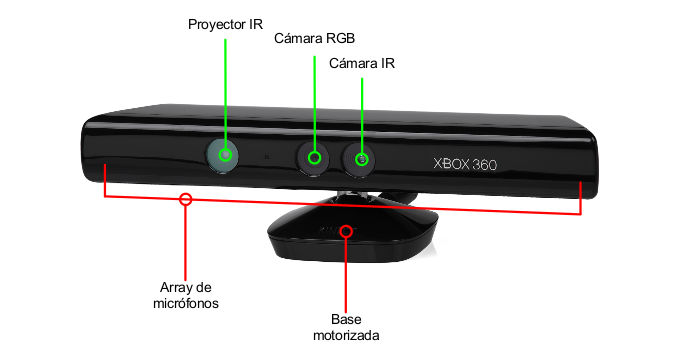
\includegraphics[width=\imsize]
{kinect}
\caption[Microsoft Kinect]
{Microsoft Kinect. Imagen original : Wikipedia bajo licencia Creative Commons\cite{wiki-kinect}.}
\label{fig:kinect}
\end{figure}

\section{Descripción}
\label{sec:descripcion-kinect}
La cámara RGB produce un \textit{stream} de datos de 24 bits por pixel, 8 bits por cada color. Su resolución estándar es 640x480 pixeles con una tasa de muestreo máxima de 30 FPS. \\
El sensor de profundidad está compuesto por un emisor láser infrarrojo (IR) y un sensor CMOS monocromo. Produce un \textit{stream} de datos de 11 bits. Posee una resolución estándar de 640x480 pixeles a una tasa de muestreo máxima de 30 FPS. \\
El campo de visión es de 57° horizontal y 43° vertical. \\
Los cámara presenta otros sensores y un mecanismo de inclinación que no fueron utilizados en este trabajo. \\

Cabe señalar que para un objeto observado en la escena, el valor de profundidad obtenido, no es la distancia real desde la Kinect al objeto, sino la distancia desde el plano del sensor (Figura \ref{fig:esquema-plano-profundidad-kinect}).

\begin{figure}[ht]
\centering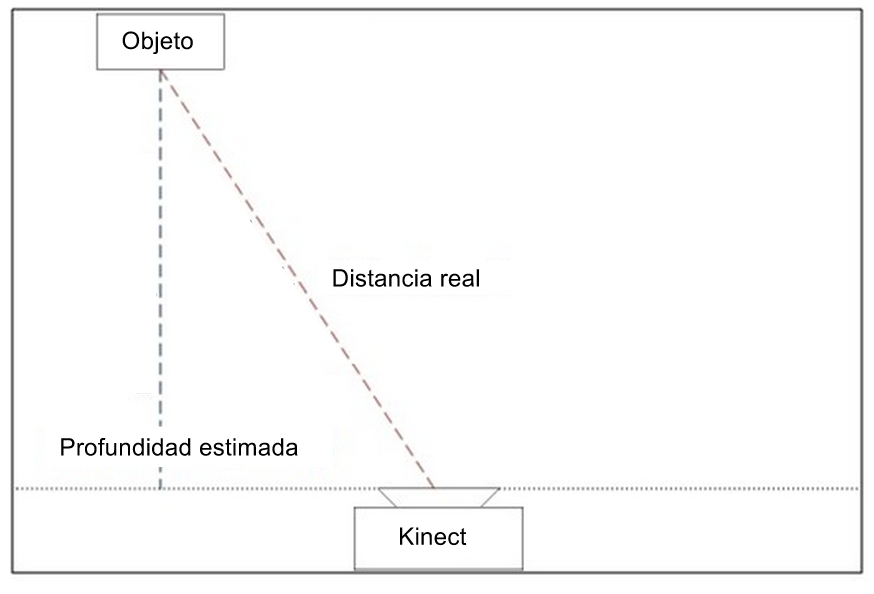
\includegraphics[width=\imsize]
{esquema-plano-profundidad-kinect}
\caption[Esquema de estimación de profundidad Kinect]
{Esquema de estimación de profundidad Kinect. Imagen original \cite{andersen12}.}
\label{fig:esquema-plano-profundidad-kinect}
\end{figure}

\section{Funcionamiento interno}
\label{sec:funcionamiento-kinect}

El funcionamiento de la cámara Kinect esta basado en tecnología propiedad de la empresa israelí PrimeSense \cite{primesense}. \\
Para obtener una imagen de profundidad el emisor láser emite un patrón de puntos que es capturado por la cámara infrarroja (sensor CMOS monocromo). Figura \ref{fig:kinect-patron-ir}. \\

\begin{figure}[ht]
\centering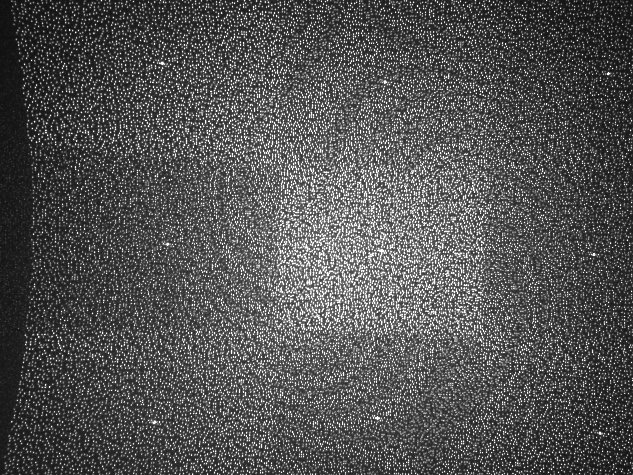
\includegraphics[width=\imsizeS]
{kinect-patron-ir}
\caption[Patrón de puntos emitido por el sensor IR]
{Patrón de puntos emitido por el sensor IR. Fuente : proyecto ROS\cite{ros} bajo licencia Creative Commons.}
\label{fig:kinect-patron-ir}
\end{figure}

El proceso que se describe en la patente de PrimeSense\cite{garcia2008range} se divide en las siguientes etapas :
\begin{enumerate}
\item Capturar el patrón de puntos para un conjunto de imágenes de referencia a diferentes distancias del plano del sensor.
\item Capturar el patrón de puntos sobre una imagen de test de la region de interes.
\item Encontrar la imagen de referencia que mayor similitud tiene con la imagen de test utilizando un método de Correlación Cruzada\cite{wiki-cross-correlation}.
\item Estimar el mapa 3D de la escena por medio de un proceso de triangulación utilizando los desplazamientos entre la imagen de test y la imagen de referencia elegida.
\end{enumerate}

En el caso del Microsoft Kinect, las imágenes de referencia han sido capturadas contra una superficie plana a distancias predefinidas y están almacenadas en el dispositivo. El sensor devuelve la imagen de profundidad en forma de valores de disparidad que luego son traducidos a distancias en metros, en un procedimiento externo, mediante la conversión :

\begin{equation}
distancia=0.1236 \cdot \tan(\frac{disparidad}{2842.5} + 1.1863)
\end{equation}

Si bien el sensor Kinect captura las imágenes RGB y de profundidad de forma independiente, en este trabajo se utiliza una librería que brinda la posibilidad de sincronizar automáticamente ambos tipos de imágenes, dando como resultado una imagen RGB-D o frame RGB-D.

\section{Consideraciones}
\label{sec:consideraciones-kinect}

En este apartado se describen algunas especificaciones para el uso del dispositivo Kinect que se consideran relevantes para este trabajo.

De acuerdo a las especificaciones oficiales, el rango de operación del sensor de profundidad se encuentra entre 0.4 m a 4 m. En Khoshelham\cite{khoshelham2011accuracy} (2011) se analiza la precisión del sensor, midiendo la profundidad de una superficie plana a diferentes distancias y se concluye que el error aleatorio de los datos de profundidad crece cuadráticamente con el aumento de la distancia entre el dispositivo y la escena observada, según se presenta en la figura \ref{fig:error-kinect}.

\begin{figure}[ht]
\centering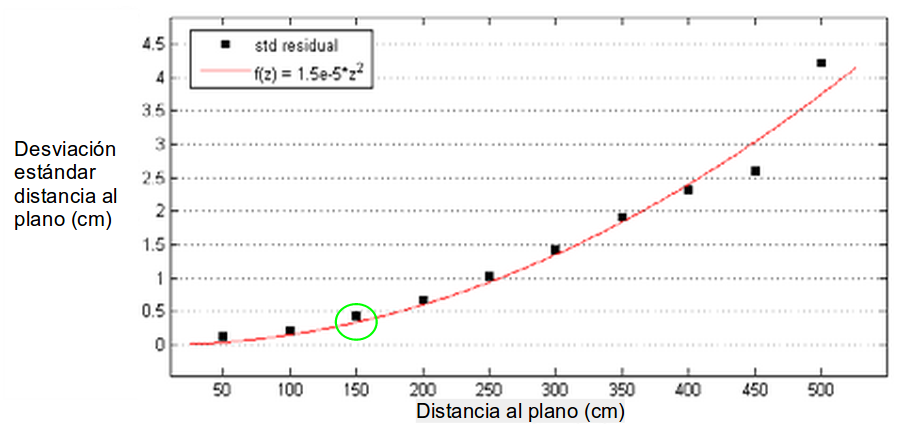
\includegraphics[width=\imsize]
{error-kinect}
\caption[Error camara Kinect]
{Desviación estándar del error en la estimación de profundidad, posicionando el sensor a diferentes distancias del plano de referencia. En rojo se muestra la curva que mejor ajusta al error. La desviación estándar presenta un valor de 0,5 cm a una distancia de 1,5 m y un maximo cercano a 4,25 cm para una distancia de 5 m. Fuente : \cite{khoshelham2011accuracy}.}
\label{fig:error-kinect}
\end{figure}

En Andersen y Ahrendt\cite{andersen12} (2012) se realiza otro análisis del sensor de profundidad del Microsoft Kinect concluyendo lo siguiente :
\begin{itemize}

\item Materiales con características reflectantes influyen sobre el sensor de profundidad imposibilitando la medición de distancias o derivando en mediciones incorrectas.

\item La luz infrarroja, en particular la luz solar, interfiere con el sensor IR limitando su utilización en entornos exteriores.

\item Debido a la distancia interna entre el emisor y el detector IR en el dispositivo Kinect, los objetos iluminados pueden provocar sombras en la imagen de fondo (Figura \ref{fig:sombra-kinect}). La sombra en el patrón imposibilita que el sensor pueda calcular la profundidad y los píxeles en el área sombreada se ponen a profundidad cero. En la figura \ref{fig:silla-sombra-kinect}, se puede observar la imagen RGB (derecha) y de profundidad (izquierda) de una silla. La cámara no pudo capturar la profundidad del borde izquierdo de silla (área en azul) debido a la posición relativa de los sensores IR con respecto a la escena.

\end{itemize}

\begin{figure}[ht]
\centering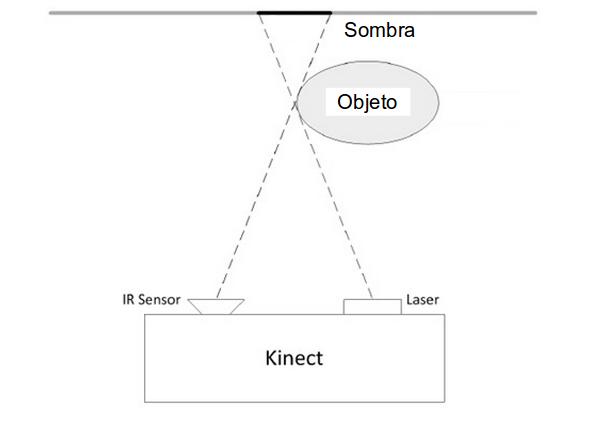
\includegraphics[width=\imsizeS]
{sombra-kinect}
\caption[Esquema de sombras en la imagen de profundidad generada por la cámara Kinect]
{Esquema de sombras en la imagen de profundidad generada por la cámara Kinect. Imagen original : \cite{andersen12}.}
\label{fig:sombra-kinect}
\end{figure}

\begin{figure}[ht]
\centering
\begin{minipage}[ht]{.45\textwidth}
\begin{center}
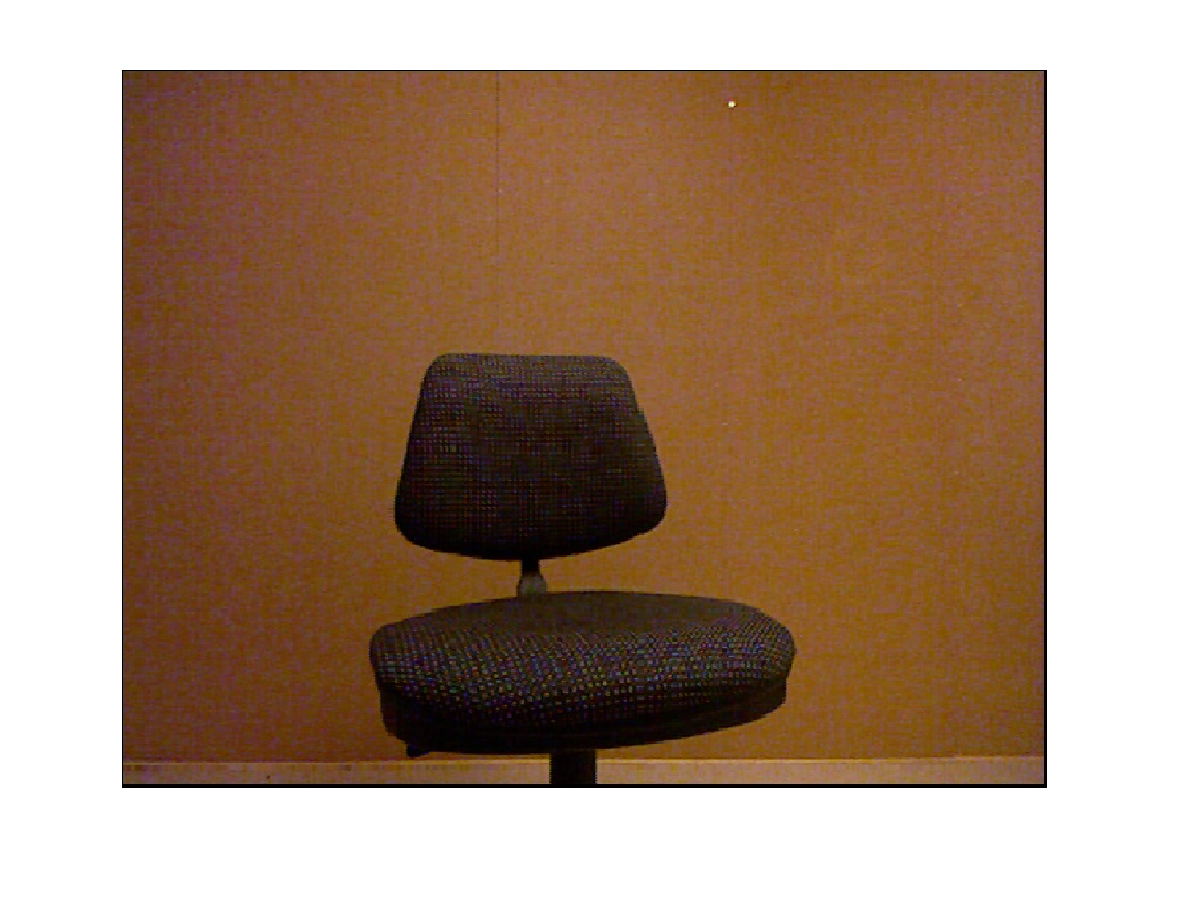
\includegraphics[width=\imsizeS]{silla-rgb-kinect}
\end{center}
\end{minipage}
\hfill
\begin{minipage}[ht]{.45\textwidth}
\begin{center}
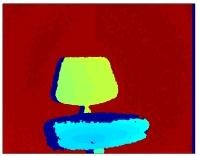
\includegraphics[width=0.91\textwidth]{silla-depth-kinect}
\end{center}
\end{minipage}
\hfill
\caption[Silla con zonas sin medición de profundidad]{Imágenes RGB (derecha) y de profundidad (izquierda) de una silla con zonas sin mediciones de profundidad (en azul). Imagen original : \cite{andersen12}.}
\label{fig:silla-sombra-kinect}
\end{figure}




\chapter{Medición de erosión en un modelo físico de laboratorio}

\section{Descripción del modelo}

Los ensayos llevados a cabo en este trabajo se realizaron en un modelo físico ubicado en el Laboratorio de Hidráulica de la Facultad de Ciencias Exactas, Físicas y Naturales (UNC). El modelo es una representación del Dique Los Molinos a escala reducida de longitudes 1:65. Este Dique se encuentra ubicado en la provincia Jujuy, sobre el río Grande, aguas debajo de la confluencia con el río Reyes. \\
El modelo físico hidráulico está representado con fondo fijo en las márgenes y fondo móvil en el lecho del río. Se representaron las obras de regulación, con todos sus componentes y elementos auxiliares de relevancia hidrosedimentológica. Cuenta con un tramo del curso fluvial con un desarrollo total de aproximadamente 1520 m (1000 m aguas arriba y 520 m aguas abajo del dique), y un ancho efectivo variable entre los 250 m a 700 m en prototipo. Estas características permiten analizar adecuadamente el comportamiento hidrosedimentológico del flujo en cercanías de las obras, el funcionamiento de las operaciones de maniobra y la erosión en el tramo de río aguas abajo del dique. Como se observa en la figura \ref{fig:modelo-fisico-dique-los-molinos}, el dique está constituido por un terraplén de materiales sueltos y dos vertederos, un tramo a nivel fijo (dique fijo), y otro regulado por 4 compuertas, conocido como dique móvil. Sobre margen derecha, se encuentra el canal moderador.

\begin{figure}[ht]
\centering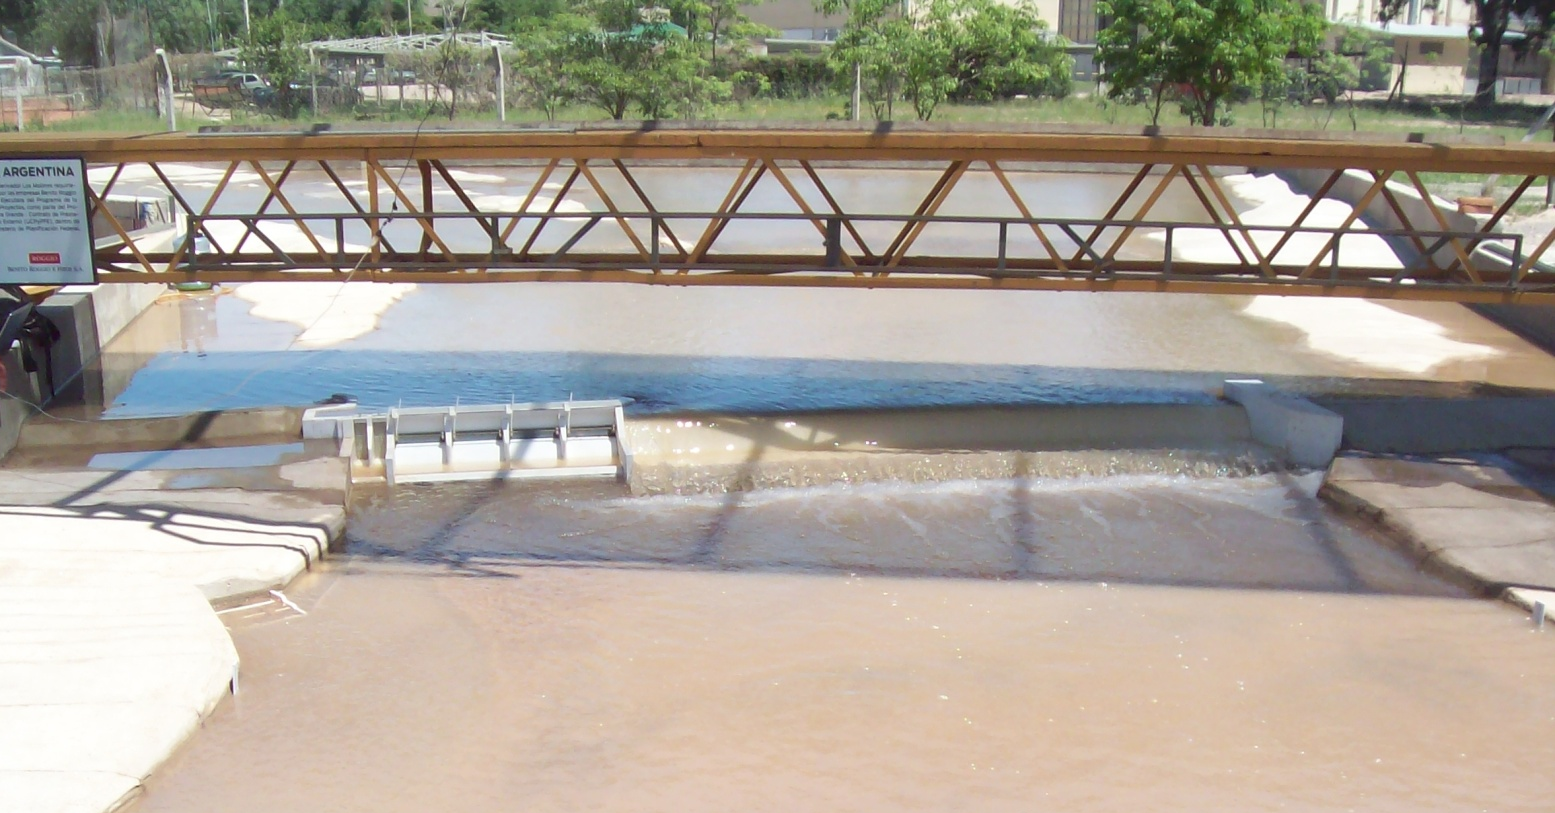
\includegraphics[width=\imsize]
{modelo-fisico-dique-los-molinos}
\caption[Modelo físico dique Los Molinos]{Modelo físico dique Los Molinos, Laboratorio de Hidráulica, FCEFyN de la UNC.}
\label{fig:modelo-fisico-dique-los-molinos}
\end{figure}

\begin{figure}[ht]

\centering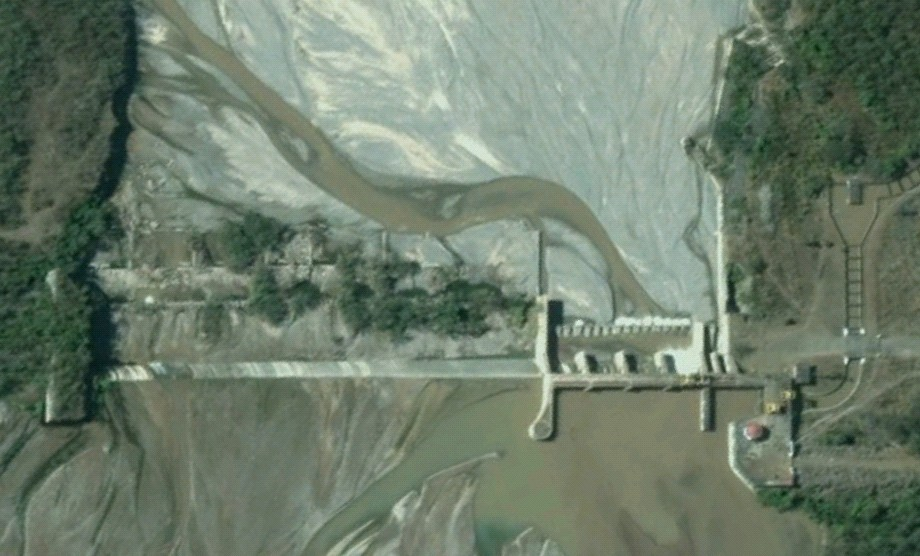
\includegraphics[width=\imsize]
{dique-los-molinos}
\caption[Dique Los Molinos]{Dique Los Molinos, Jujuy.}
\label{fig:dique-los-molinos}

\end{figure}

Teniendo en cuenta el alcance de este trabajo, los objetivos para el estudio sobre este modelo fueron los siguientes:
\begin{itemize}

\item Analizar y cuantificar las erosiones locales, aguas abajo de las estructuras de descarga a los fines de constatar el funcionamiento de las obras previstas en el proyecto. Esta evaluación se llevará a cabo para escenarios hidrológicos de diseño.

\item Verificar y optimizar las consignas de operación de las estructuras de control, a los fines de regular los procesos hidrosedimentológicos frente a crecientes aguas arriba del dique móvil.

\end{itemize}

Sobre la zona relevante, se ha construido una plataforma móvil que posibilita realizar las mediciones de erosión. Figura \ref{fig:sistema-camara-carro}. Sus componentes principales son:

\begin{itemize}

\item Un puente grúa. Este puede ser trasladado para observar distintas áreas del modelo.

\item Una guía-riel y un carro-soporte para la cámara Kinect. La guía se anexa al puente grúa, lo que permite la traslación de la cámara a lo ancho del modelo.

\end{itemize}

\begin{figure}[ht]
\centering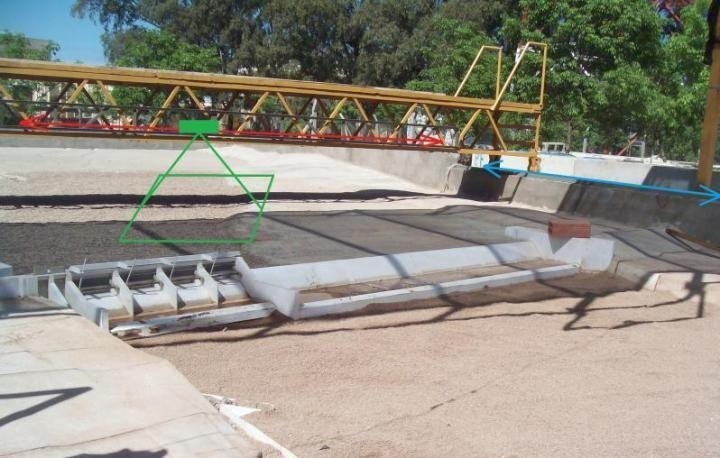
\includegraphics[width=\imsize]
{esquema-camara-puente-grua}
\caption[Puente grúa]{Puente grúa. Las flechas indican la direcciones en la que se puede trasladar la cámara (esquematizada con el recuadro verde). En rojo, traslación utilizando el carro soporte, mientras que la trayectoria en azul, se consigue movilizando el puente grúa.}
\label{fig:esquema-camara-puente-grua}
\end{figure}

\begin{figure}[ht]
\centering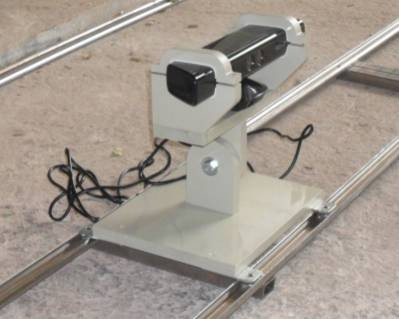
\includegraphics[width=\imsizeS]
{sistema-camara-carro}
\caption[Sistema cámara-soporte]{Soporte construido para trasladar la cámara sobre el modelo.}
\label{fig:sistema-camara-carro}
\end{figure}

%%%%%%%%%%%%%%%%%%%%%%%%%%%%%%%%%%%%%%%%%%%%%%%%%%%%%%%%%%%%%%%%%%%%%%%%%%%%%%%

\section{Etapas de un ensayo hidráulico}
\label{sec:etapas-previas-medicion}

En cada ensayo hidráulico realizado, se cubrieron las etapas enumeradas a continuación:  
\begin{enumerate}

\item Se estableció la condición inicial del modelo, aguas abajo de las estructuras, nivelando el material suelto (arena) hasta la cota del terreno medido con la topografía provista. Figura \ref{fig:condicion-inicial-modelo}. Se utilizó una cota media de 1360 m s.n.m.

\item Encendido del modelo. Se encienden las bombas hidráulicas y comienza a recircular el agua dentro de cisternas y canales de aforos del laboratorio. Se realiza un manejo del sistema de bombeo hasta alcanzar el caudal establecido para cada  ensayo o escenario a simular.

\item Monitoreo de la erosión durante cada ensayo hasta alcanzar la condición de estabilidad. Estas mediciones se llevan a cabo con nivel óptico y mira. Se realizan mediciones de nivel en las zonas de interés durante intervalos temporales regulares, hasta medir valores similares entre estos intervalos.

\item Apagado del modelo. Se apagan las bombas hidráulicas, se cierran las compuertas correspondientes, y se deja drenar el modelo.

\item Medición de erosión. Esta etapa se desarrollará en detalle en las siguientes secciones.

\end{enumerate}

\begin{figure}[ht]
\centering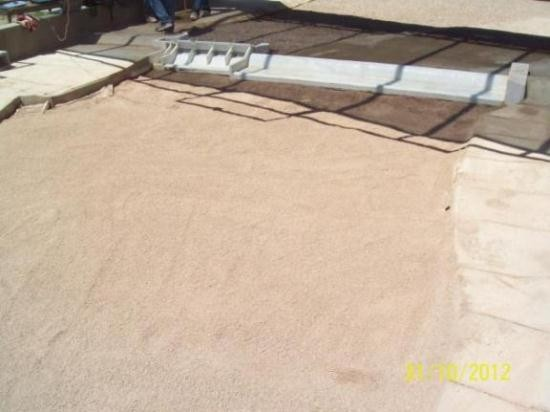
\includegraphics[width=\imsizeS]
{condicion-inicial-modelo}
\caption[Condición inicial del modelo]
{Condición inicial del modelo}
\label{fig:condicion-inicial-modelo}
\end{figure}

%%%%%%%%%%%%%%%%%%%%%%%%%%%%%%%%%%%%%%%%%%%%%%%%%%%%%%%%%%%%%%%%%%%%%%%%%%%%%%%

\section{Metodología de medición con nivel óptico}

La técnica tradicional consiste en el relevamiento manual de puntos sobre perfiles longitudinales y transversales (en la figura \ref{fig:esquema-perfiles}), por lo general cada 10 cm, utilizando para dicha tarea el nivel óptico (en la figura \ref{fig:nivel-optico}) y una mira con una escala graduada al milímetro.  

\begin{figure}[ht]
\centering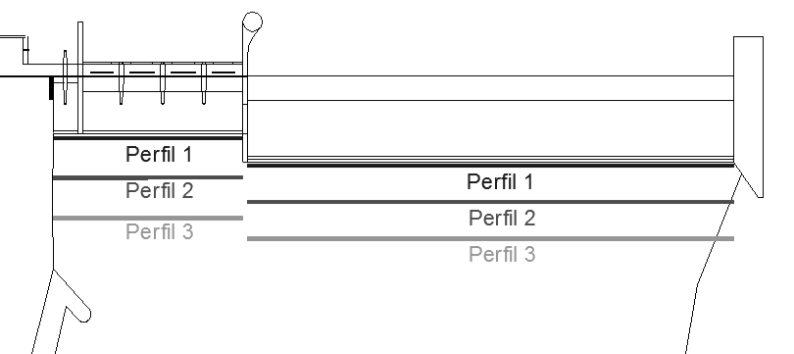
\includegraphics[width=\imsize]
{esquema-perfiles}
\caption[Perfiles transversales]
{Ubicación de perfiles transversales para medir las erosiones finales.}
\label{fig:esquema-perfiles}
\end{figure}

\begin{figure}[ht]
\centering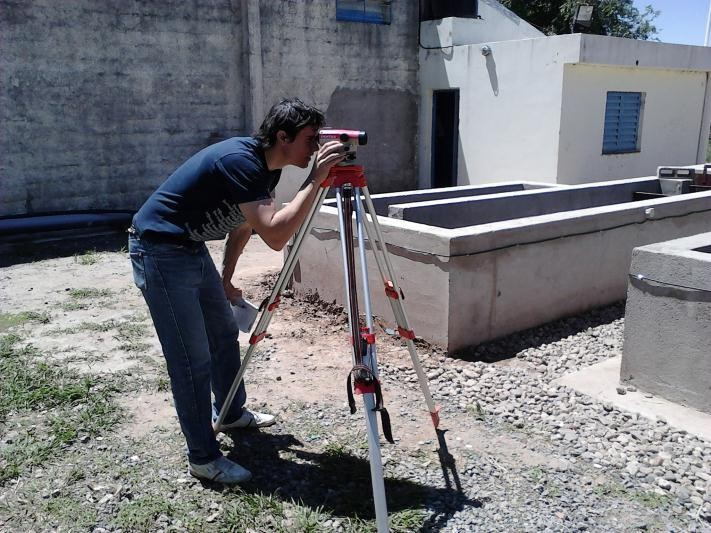
\includegraphics[width=\imsize]
{nivel-optico}
\caption[Nivel óptico]
{Medición con nivel óptico en modelo físico Los Molinos, cortesía de Nicolás Bellino.}
\label{fig:nivel-optico}
\end{figure}

Por último, se realiza la digitalización manual y conversión de modelo a prototipo de los puntos relevados. \\
Cabe destacar que para implementar esta técnica suelen participar 3 personas e invertir aproximadamente 20 minutos por cada metro cuadrado, relevando puntos cada 15 cm.
\section{Metodología de medición con cámara RGB-D}
\label{sec:metodologia-medicion-digital}

En esta sección, se describe la aplicación de la técnica digital de medición de erosión propuesta en este trabajo. \\

Se tuvieron en cuenta un conjunto de consideraciones que forman parte de la técnica de medición y permiten obtener resultados óptimos, las cuales se presentan a continuación:

\begin{itemize}

\item La superficie a relevar debe estar libre de agua. Como se mencionó en el apartado \ref{sec:consideraciones-kinect}, se observó que los objetos con características reflectantes afectan al sensor de profundidad de la Kinect. Figura \ref{fig:modelo-condiciones-agua}.

\item La escena debe estar al resguardo de la luz solar, como se explica en el apartado \ref{sec:consideraciones-kinect}. Debido a que el modelo físico utilizado se encuentra al aire libre, en el exterior del Laboratorio de Hidráulica, fue necesario utilizar un nailon de color negro colocado sobre el puente grúa, como se puede observar en la figura \ref{fig:modelo-lona}. Alternativamente, se consideró realizar las mediciones al atardecer cuando la luz solar es más tenue. Se concluye que utilizando el nailon se obtienen condiciones lumínicas estables, quitando así una restricción para el horario de medición.

\item La guía debe estar horizontalizada. El plano desde el que se captura la escena debe estar a una altitud constante para que la representación de la superficie sea consistente. Esta condición debe ser verificada al iniciar cada ensayo hidráulico.

\item La cámara debe ubicarse en un rango de 0.4 m  a 1.5 m de altura sobre la escena a relevar, para que el error de medición se mantenga dentro del intervalo aceptable (aproximadamente 5 mm), según el análisis del sensor Kinect presentado en el apartado \ref{sec:consideraciones-kinect}.

\end{itemize}

\begin{figure}[ht]
\centering
\begin{minipage}[t]{.45\textwidth}
\begin{center}
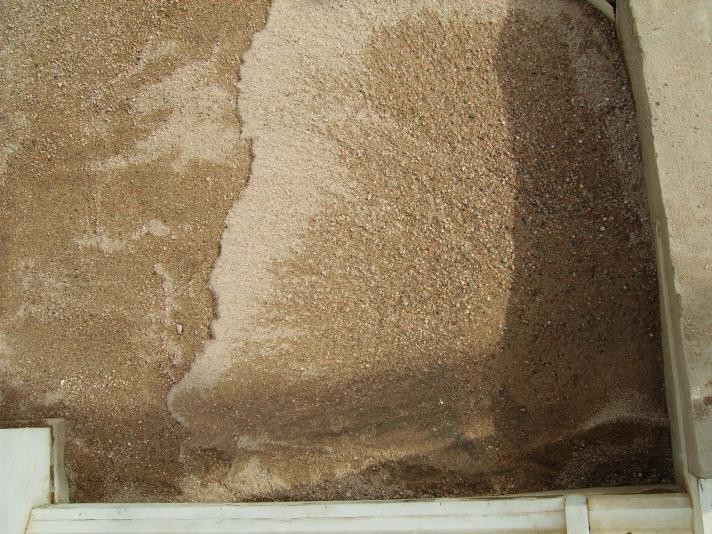
\includegraphics[width=\imsizeS]{modelo-sin-agua} % primera imagen colocada a la izquierda
\end{center}
\end{minipage}
\hfill
\begin{minipage}[t]{.45\textwidth}
\begin{center}
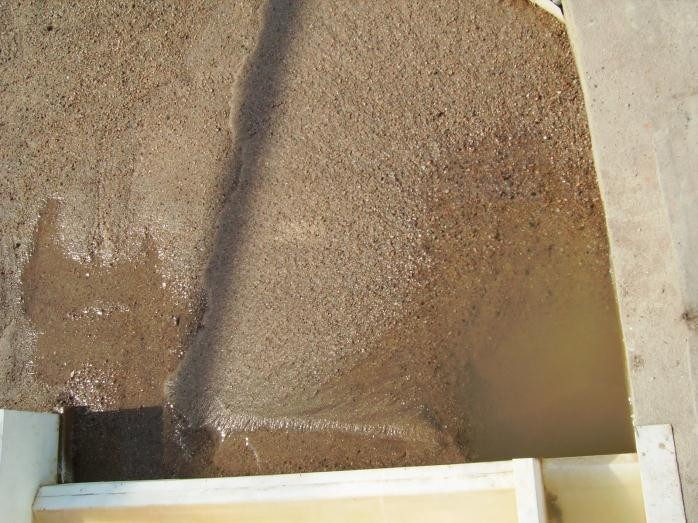
\includegraphics[width=\imsizeS]{modelo-con-agua} % segunda imagen colocada a la derecha
\end{center}
\end{minipage}
\hfill
\caption[Modelo físico con y sin agua sobre la superficie]{Derecha: condición correcta para la medición. Izquierda: se observan espejos de agua que interfieren el sensor infrarrojo de la cámara.}
\label{fig:modelo-condiciones-agua}
\end{figure}

\begin{figure}[ht]
\centering
\begin{minipage}[t]{.45\textwidth}
\begin{center}
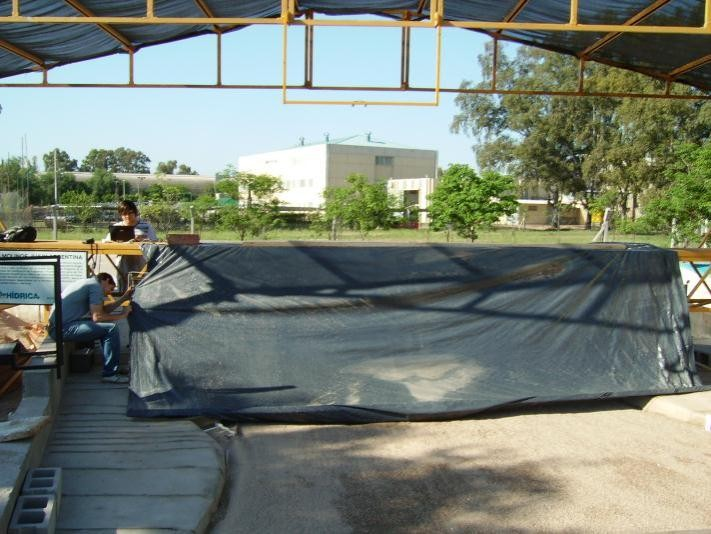
\includegraphics[width=\imsizeS]{modelo-lona1} % primera imagen colocada a la izquierda
\end{center}
\end{minipage}
\hfill
\begin{minipage}[t]{.45\textwidth}
\begin{center}
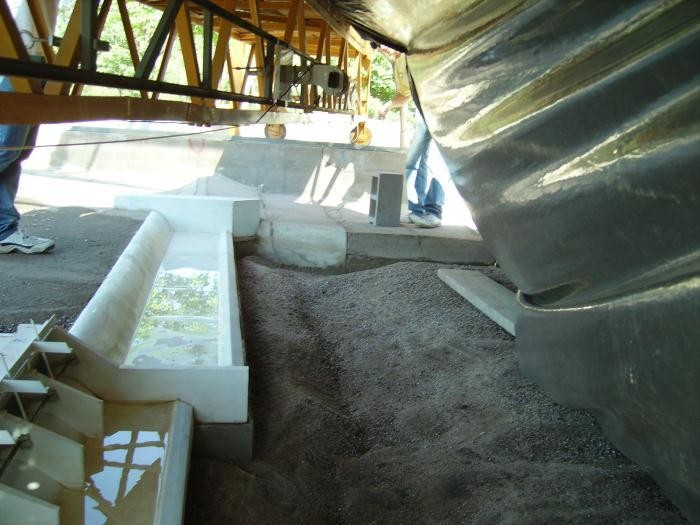
\includegraphics[width=\imsizeS]{modelo-lona2} % segunda imagen colocada a la derecha
\end{center}
\end{minipage}
\hfill
\caption[Nailon utilizado para evitar interferencia de luz solar]{Derecha: Forma de colocar el nailon sobre el puente grúa para cubrir todo el largo del riel. Izquierda: La sombra producida por el nailon permite capturar las imágenes sin interferencia del sol.}
\label{fig:modelo-lona}
\end{figure}

Habiendo verificado las condiciones anteriores, se introduce el carro-soporte en el carril-guía y se inicia la aplicación de registración \textit{ModelMapper} \ref{sec:model-mapper}. \\
 
En la figura \ref{fig:aguas-abajo-desplazamiento-carro}, se observa cómo manipular la plataforma móvil para capturar la escena. Se propone un desplazamiento del carro de aproximadamente 40 cm entre cada captura, para que el área superpuesta entre dos nubes puntos consecutivas esté próxima al 50\%. Si la aplicación no lograr realizar la registración correctamente se corrige la ubicación del sensor a una posición intermedia.

\begin{figure}[ht]
\centering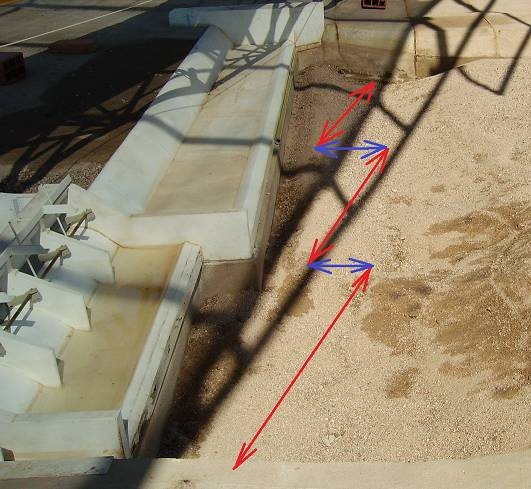
\includegraphics[width=\imsize]
{aguas-abajo-desplazamiento-carro}
\caption[Desplazamiento de la cámara]{Recorrido del puente grúa y del carro-soporte sobre la escena. Las flechas rojas indican desplazamiento de la cámara y las flechas azules representan el movimiento del puente.}
\label{fig:aguas-abajo-desplazamiento-carro}
\end{figure}

En el apartado \ref{sec:conversion-mapa3D-prototipo} se describe que para realizar la conversión a prototipo es necesario un punto fijo con cotas conocidas en los sistemas del modelo y del prototipo. Con este fin, se recomienda que la escena capture las estructuras fijas en el modelo físico con medidas de elevación dada por mediciones topográficas. En caso contrario, se puede medir con nivel óptico un punto visible en la escena y utilizar su cota prototipo como referencia. \\
Utilizando la técnica digital se invierte aproximadamente 1 min para trasladar la cámara y procesar un nuevo frame. Teniendo en cuenta que se requieren 6 frames (aprox.) por $m^{2}$ y posiblemente se descarte algún frame en el proceso, se estiman 10 min para relevar un área de un $m^{2}$. Comparando con la técnica tradicional, se observa que se reduce por la mitad el tiempo invertido para cada ensayo.

%%%%%%%%%%%%%%%%%%%%%%%%%%%%%%%%%%%%%%%%%%%%%%%%%%%%%%%%%%%%%%%%%%%%%%%%%%%%%%%

\section{Ensayos realizados}
En la tabla siguiente se presenta un resumen de los ensayos realizados. Se detallan los caudales asociados así como las estructuras hidráulicas por las que pasa cada uno y su representatividad.\\

\begin{tabular}{ccc}
\hline
Ensayo  & Caudal total $m^{3}/s$ & Motivación \\
\hline
1 & 900 & Caudal Máximo Dique Móvil (DM) y \\
  &     & Canal Moderador (CM) \\
\hline
2 & 3200 & Caudal Máximo Sólo Dique Fijo (DF) \\
\hline
3,7,9 & 4200 & Caudal para Periodo de Retorno T=10000 años \\
\hline
4 & 90 & Caudal de Despegue CM \\
\hline
5 & 225 & Caudal de Despegue DM \\
\hline
10 & 600 & Caudal de Verificación DF, DM y CM
 \\
\hline
13 & 1600 & Caudal de Verificación DF, DM y CM
 \\
\hline
14 & 600 & Caudal de Verificación DM y CM
 \\
\hline
\end{tabular}

\newpage % Salto de página para acomodar las imágenes

\subsection{Medición de erosión máxima}
\label{sec:ensayo-erosion-maxima}

En el ámbito de la Ingeniería Civil, la representación con modelos físicos a escala reducida y la simulación de ensayos hidráulicos fluviales, como los que aquí se presentan, tiene entre sus objetivos principales definir las cotas de erosión máxima. Estas mediciones se realizan con el fin de establecer las profundidades de fundación de los muros de contención de las estructuras hidráulicas que componen el sistema evaluado. \\
Se muestran los mapas de elevación en escala prototipo, generados a partir del relevamiento de fosos de erosión ubicados aguas abajo de las estructuras, para los ensayos 1 y 3. Como punto de referencia se utilizó la parte superior del dique móvil, con cota igual a 1377.77 m s.n.m.\\

\begin{figure}[ht]
\centering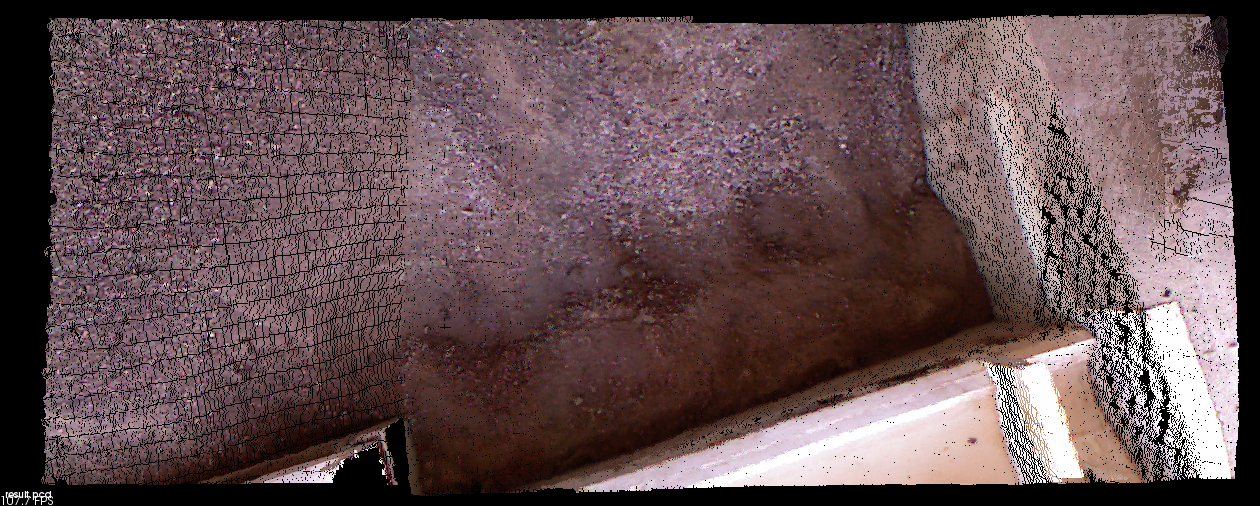
\includegraphics[width=\imsizeL]
{Q900_rgb}
\caption[Imagen RGB Ensayo 1]
{Ensayo 1. Foso de erosión aguas abajo del dique móvil.  Imagen RGB.}
\label{fig:Q900_rgb}
\end{figure}

\begin{figure}[ht]
\centering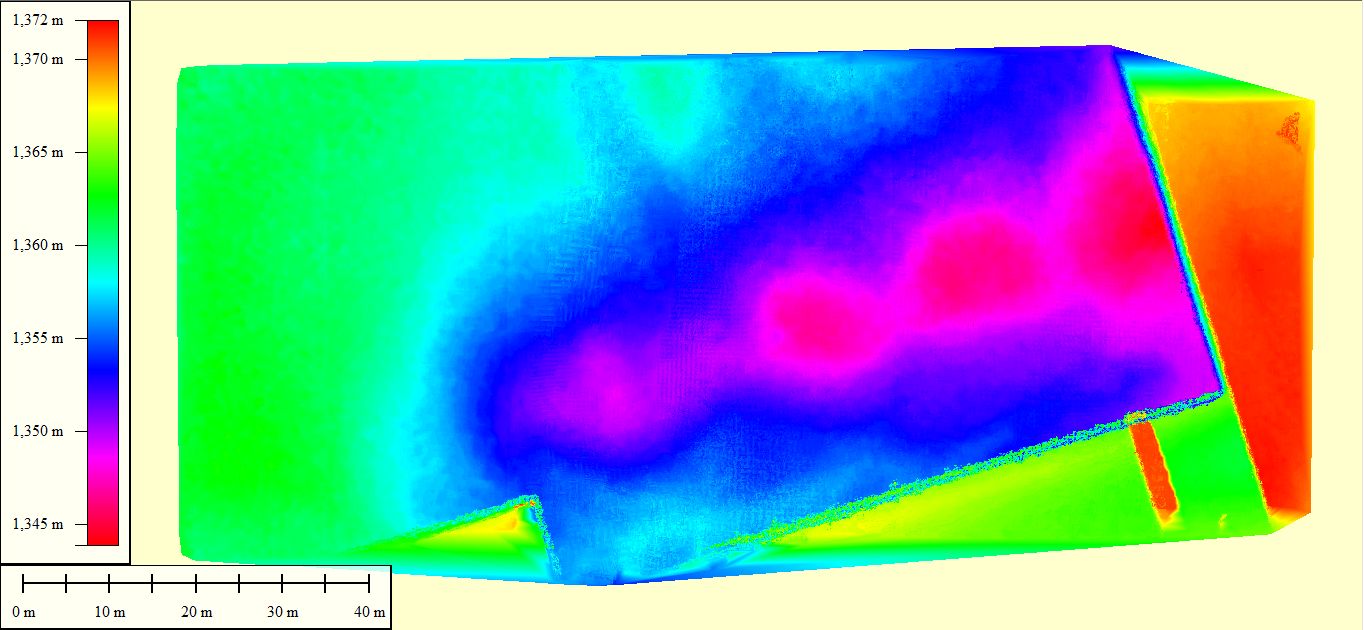
\includegraphics[width=\imsizeL]
{Q900_dem}
\caption[DEM Ensayo 1]
{Ensayo 1. Foso de erosión aguas abajo del dique móvil. Modelo digital de elevaciones.}
\label{fig:Q900_dem}
\end{figure}

\begin{figure}[ht]
\centering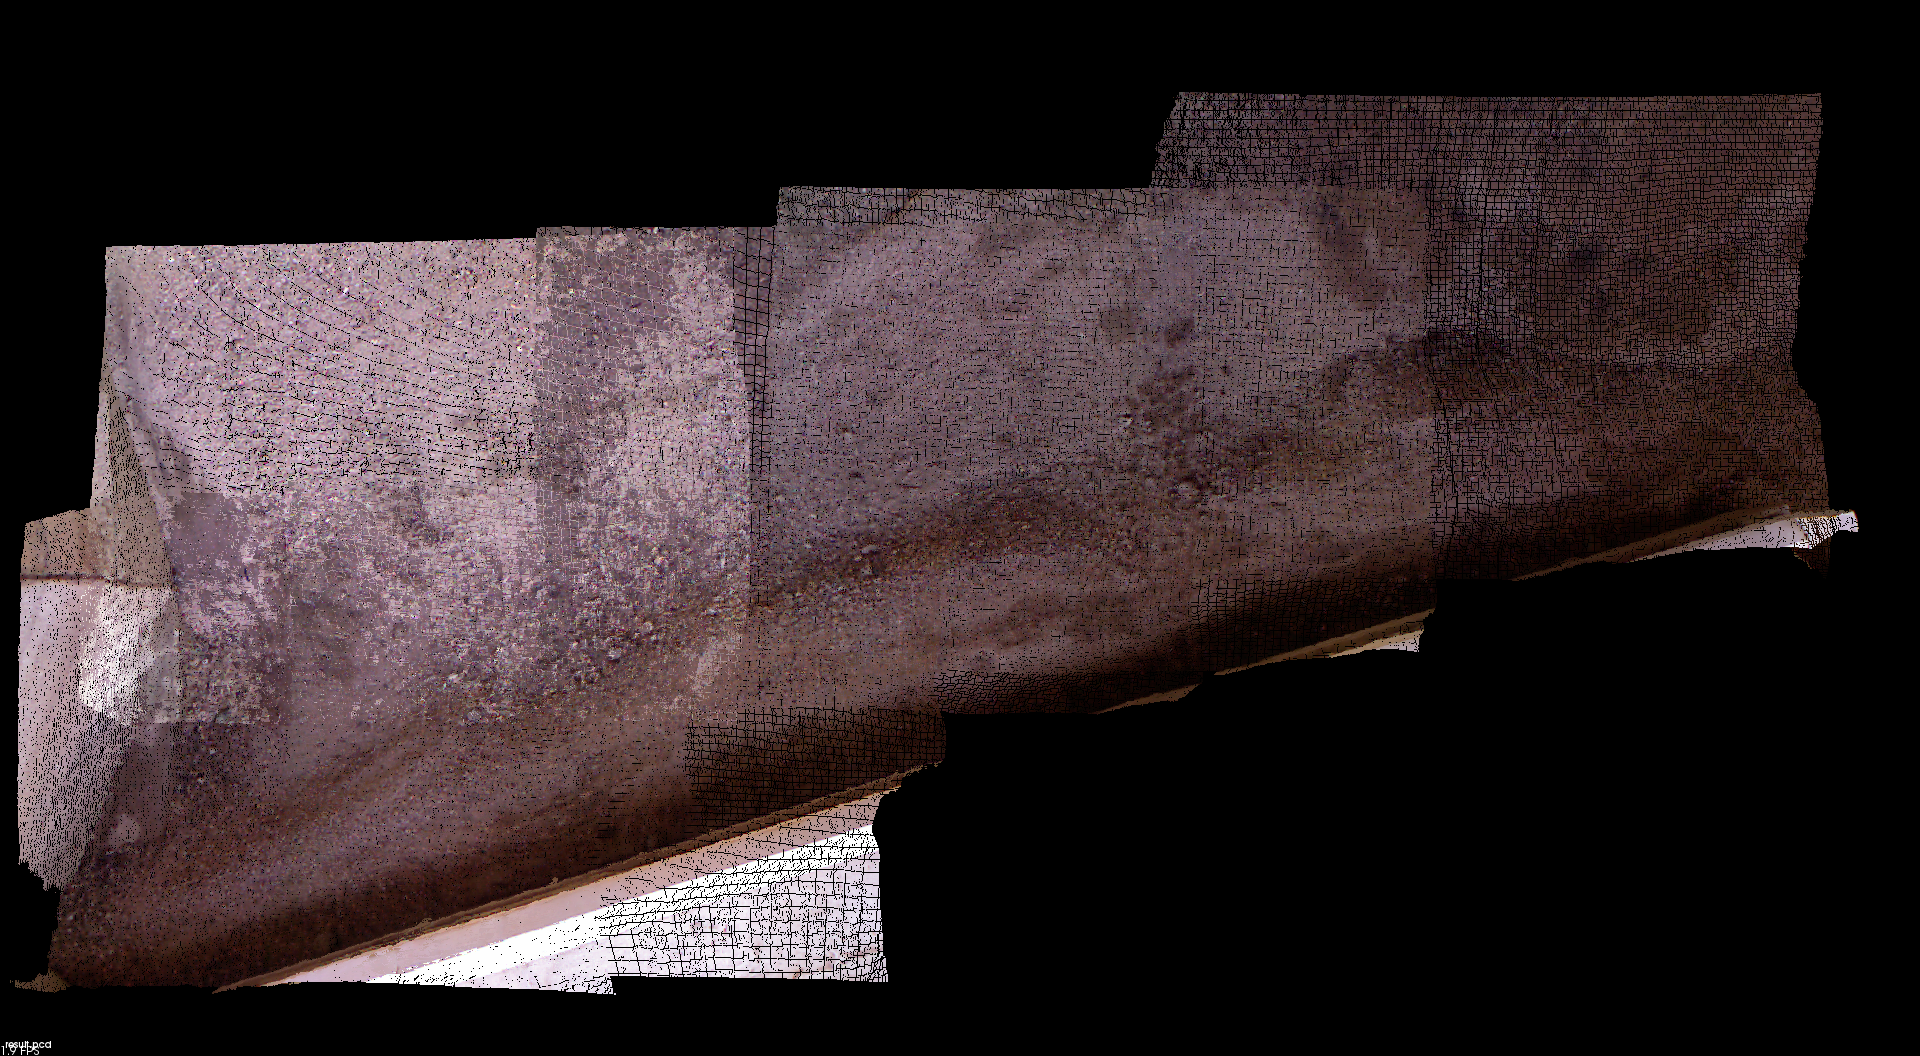
\includegraphics[width=\imsizeL]
{Q4200_rgb}
\caption[Imagen RGB Ensayo 3]
{Ensayo 3. Foso de erosión aguas abajo del dique fijo. Imagen RGB.}
\label{fig:Q4200_rgb}
\end{figure}

\begin{figure}[ht]
\centering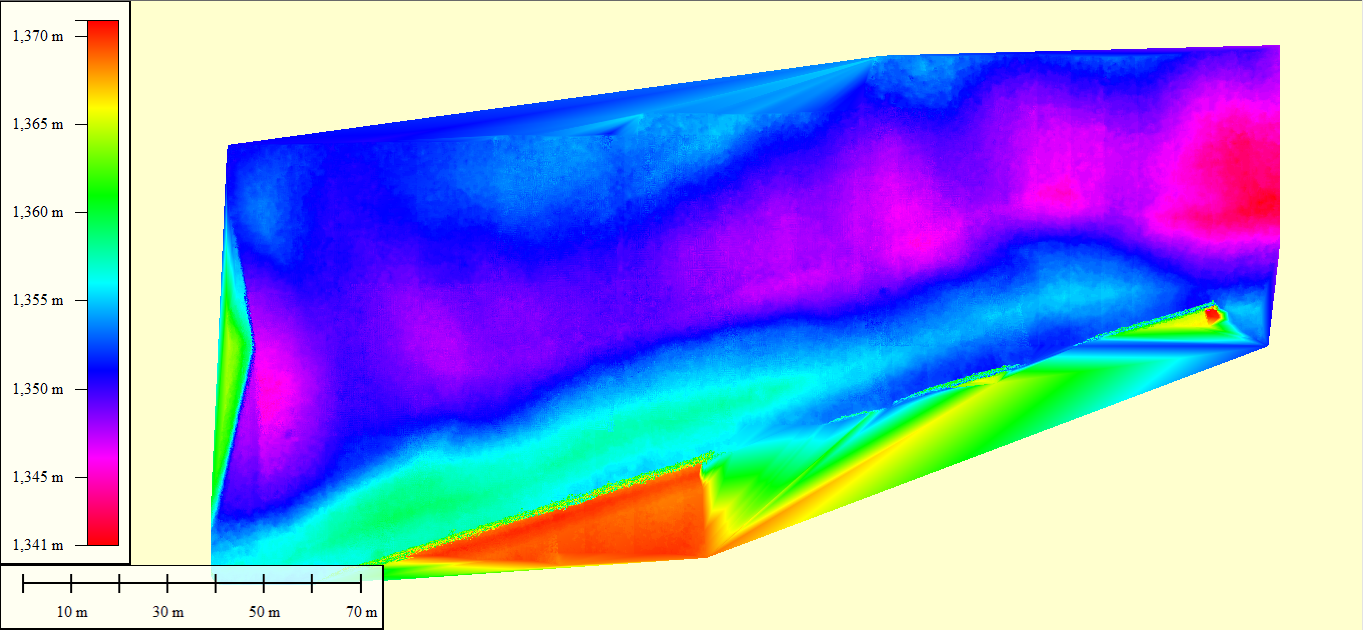
\includegraphics[width=\imsizeL]
{Q4200_dem}
\caption[DEM Ensayo 3]
{Ensayo 1. Foso de erosión aguas abajo del dique fijo. Modelo digital de elevaciones.}
\label{fig:Q4200_dem}
\end{figure}

\subsection{Medición de formas de fondo}
\label{sec:ensayo-formas-de-fondo}

Estas mediciones se realizaron con el objetivo de verificar y optimizar las consignas de operación de las estructuras de control, con el fin de regular los procesos hidrosedimentológicos presentes en las proximidades de la presa aguas arriba.\\
En este ensayo se relevaron las canalizaciones hacia las compuertas del dique móvil y el canal moderador. El análisis de los canales que se formaron sobre la superficie del modelo, debido a las llamadas que se realiza con la operación de las estructuras de control, requiere relevar una densidad de puntos elevada y a la vez cubrir grandes áreas de superficie. La técnica digital aborda esta tarea de forma mucha más eficiente y precisa que la metodología tradicional. \\
Se muestran los mapas de elevación en escala prototipo, generados a partir del área de modelación aguas arriba del dique, para el ensayo 10. Como punto de referencia se utilizó la parte superior del dique móvil, con cota igual a 1377.77 m s.n.m.

\begin{figure}[ht]
\centering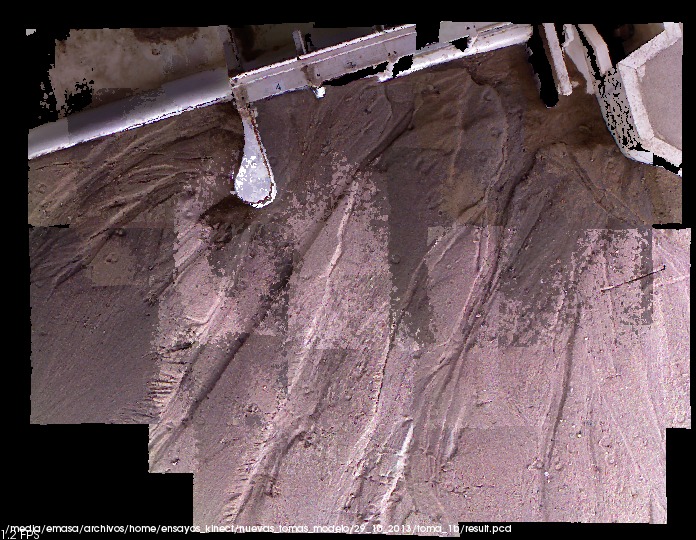
\includegraphics[width=\imsizeL]
{Q600_rgb}
\caption[Imagen RGB Ensayo 10]
{Ensayo 10. Área aguas arriba del dique móvil. Imagen RGB.}
\label{fig:Q600_rgb}
\end{figure}

\begin{figure}[ht]
\centering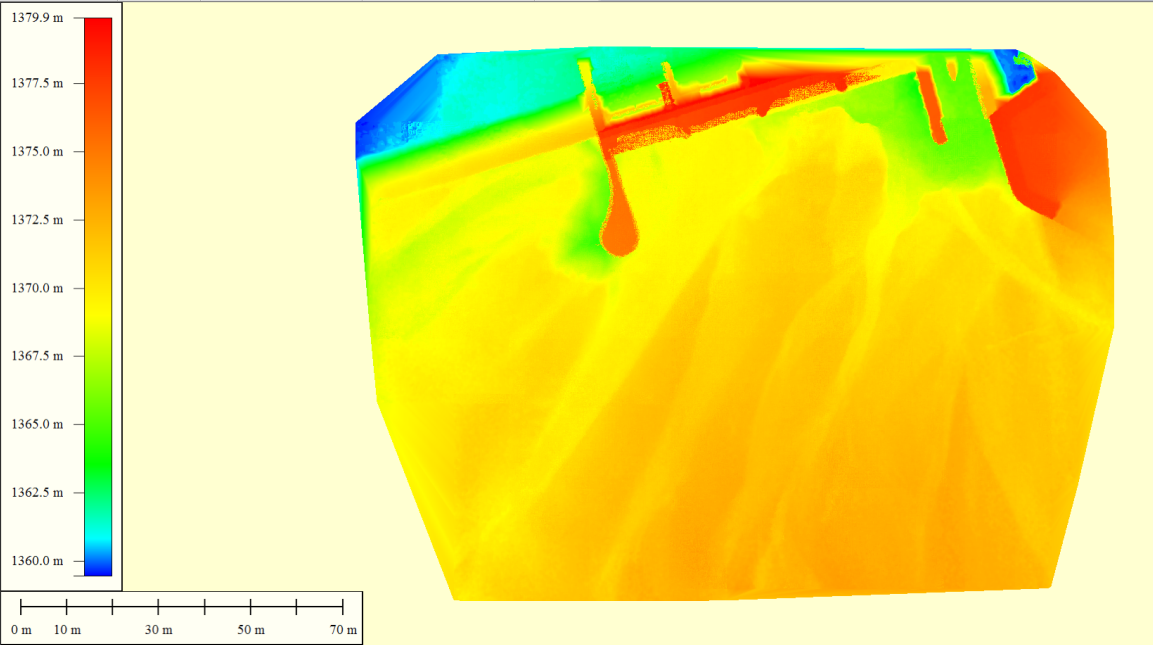
\includegraphics[width=\imsizeL]
{Q600_dem}
\caption[DEM Ensayo 10]
{Ensayo 10. Área aguas arriba del dique móvil. Modelo digital de elevaciones.}
\label{fig:Q600_dem}
\end{figure}

\chapter{Análisis de los resultados}
En este capítulo se analizan varios aspectos de la técnica digital en contraste con la técnica tradicional buscando validar la solución propuesta y demostrar las ventajas que esta presenta.

\section{Comparación de perfiles}
Utilizando los resultados presentados en los ensayos \ref{sec:ensayo-erosion-maxima}, se comparan perfiles obtenidos con ambas técnicas con el objetivo de estudiar la bondad de la técnica digital para relevar la condición de erosión. \\
En la figura \ref{fig:comparacion-perfiles}, se muestran tres perfiles sobre el foso de erosión capturados con las tecnicas digital y tradicional. \\
En el perfil superior izquierdo, se observa que los datos continuos relevados con la cámara son aproximados de forma precisa por las mediciones con nivel óptico en condiciones donde el terreno no presenta cambios abruptos. \\
En el perfil superior derecho, se observan 3 mediciones, a 30 m, 42 m y 60 m respectivamante, que se presumen haber sido tomadas de forma incorrecta con el nivel optico. No obstante, sirve para ilustrar que la tecnica tradicional puede sufrir de errores de hasta 15 mm en prototipo, o equivalentemente, 1 m en prototipo (utilizando una escala 1:65) que no podrian ser detectados sin una superficie de referencia. Aproximadamente a los 50 m se incurre en un error de una indole distinta. En este caso, la causa de la medicion incorrecta es un cambio abrupto en la condicion del terreno, que no pudo ser detectada por el operador de la mira debido la escala del modelo. \\ 
En última instancia, se presenta el perfil inferior donde se observa el efecto de la pendiente del foso de erosión sobre una serie de mediciones con nivel. En este caso, la pendiente dificulta el apoyo del palpador sobre la superficie sin producir alteraciones, derivando en mediciones por encima del valor real. \\
Estas comparaciones ponen en evidencia que la resolución del modelo 3D obtenido con la técnica digital, es superior en zonas donde los datos relevados con la técnica tradicional no han sido cuidadosamente elegidos o el terreno es muy irregular. Cuando estos errores no están presentes, la precisión de ambas técnicas se encuentra similar.

\begin{figure}[ht]
\centering
\begin{minipage}[h]{.45\textwidth}
\begin{center}
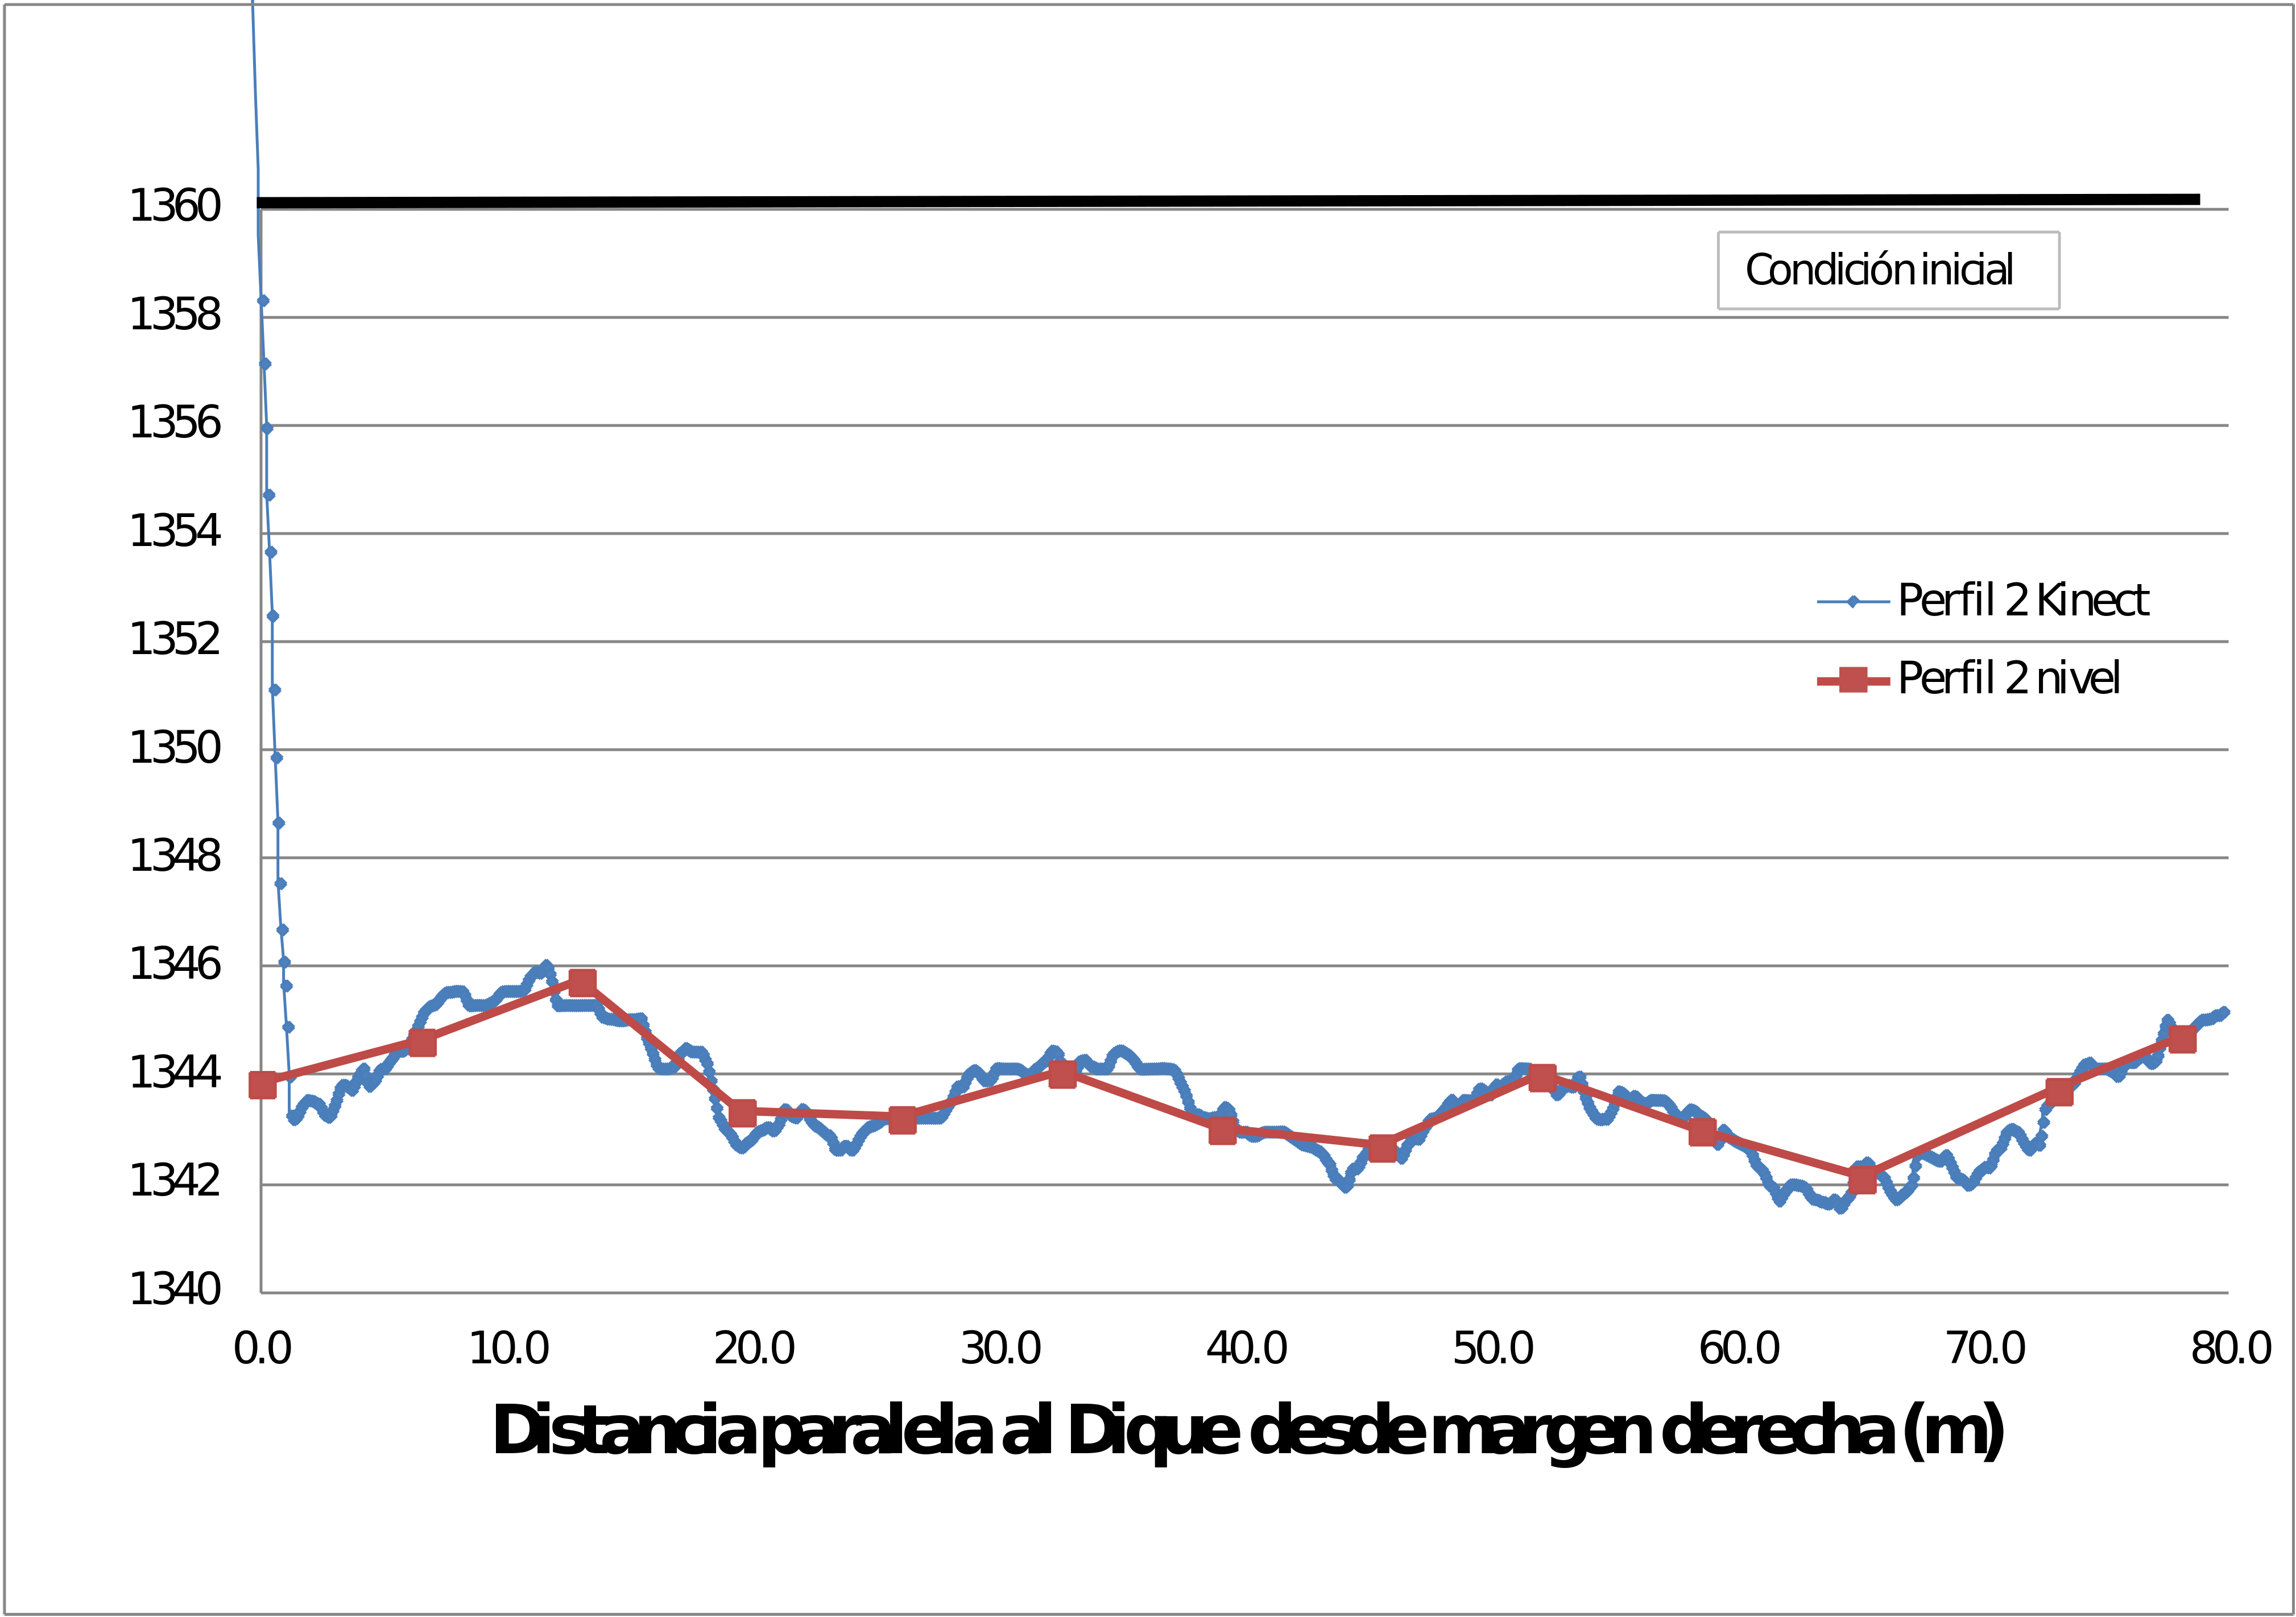
\includegraphics[width=\imsizeS]{foso-erosion-izquierda}
\end{center}
\end{minipage}
\hfill
\begin{minipage}[h]{.45\textwidth}
\begin{center}
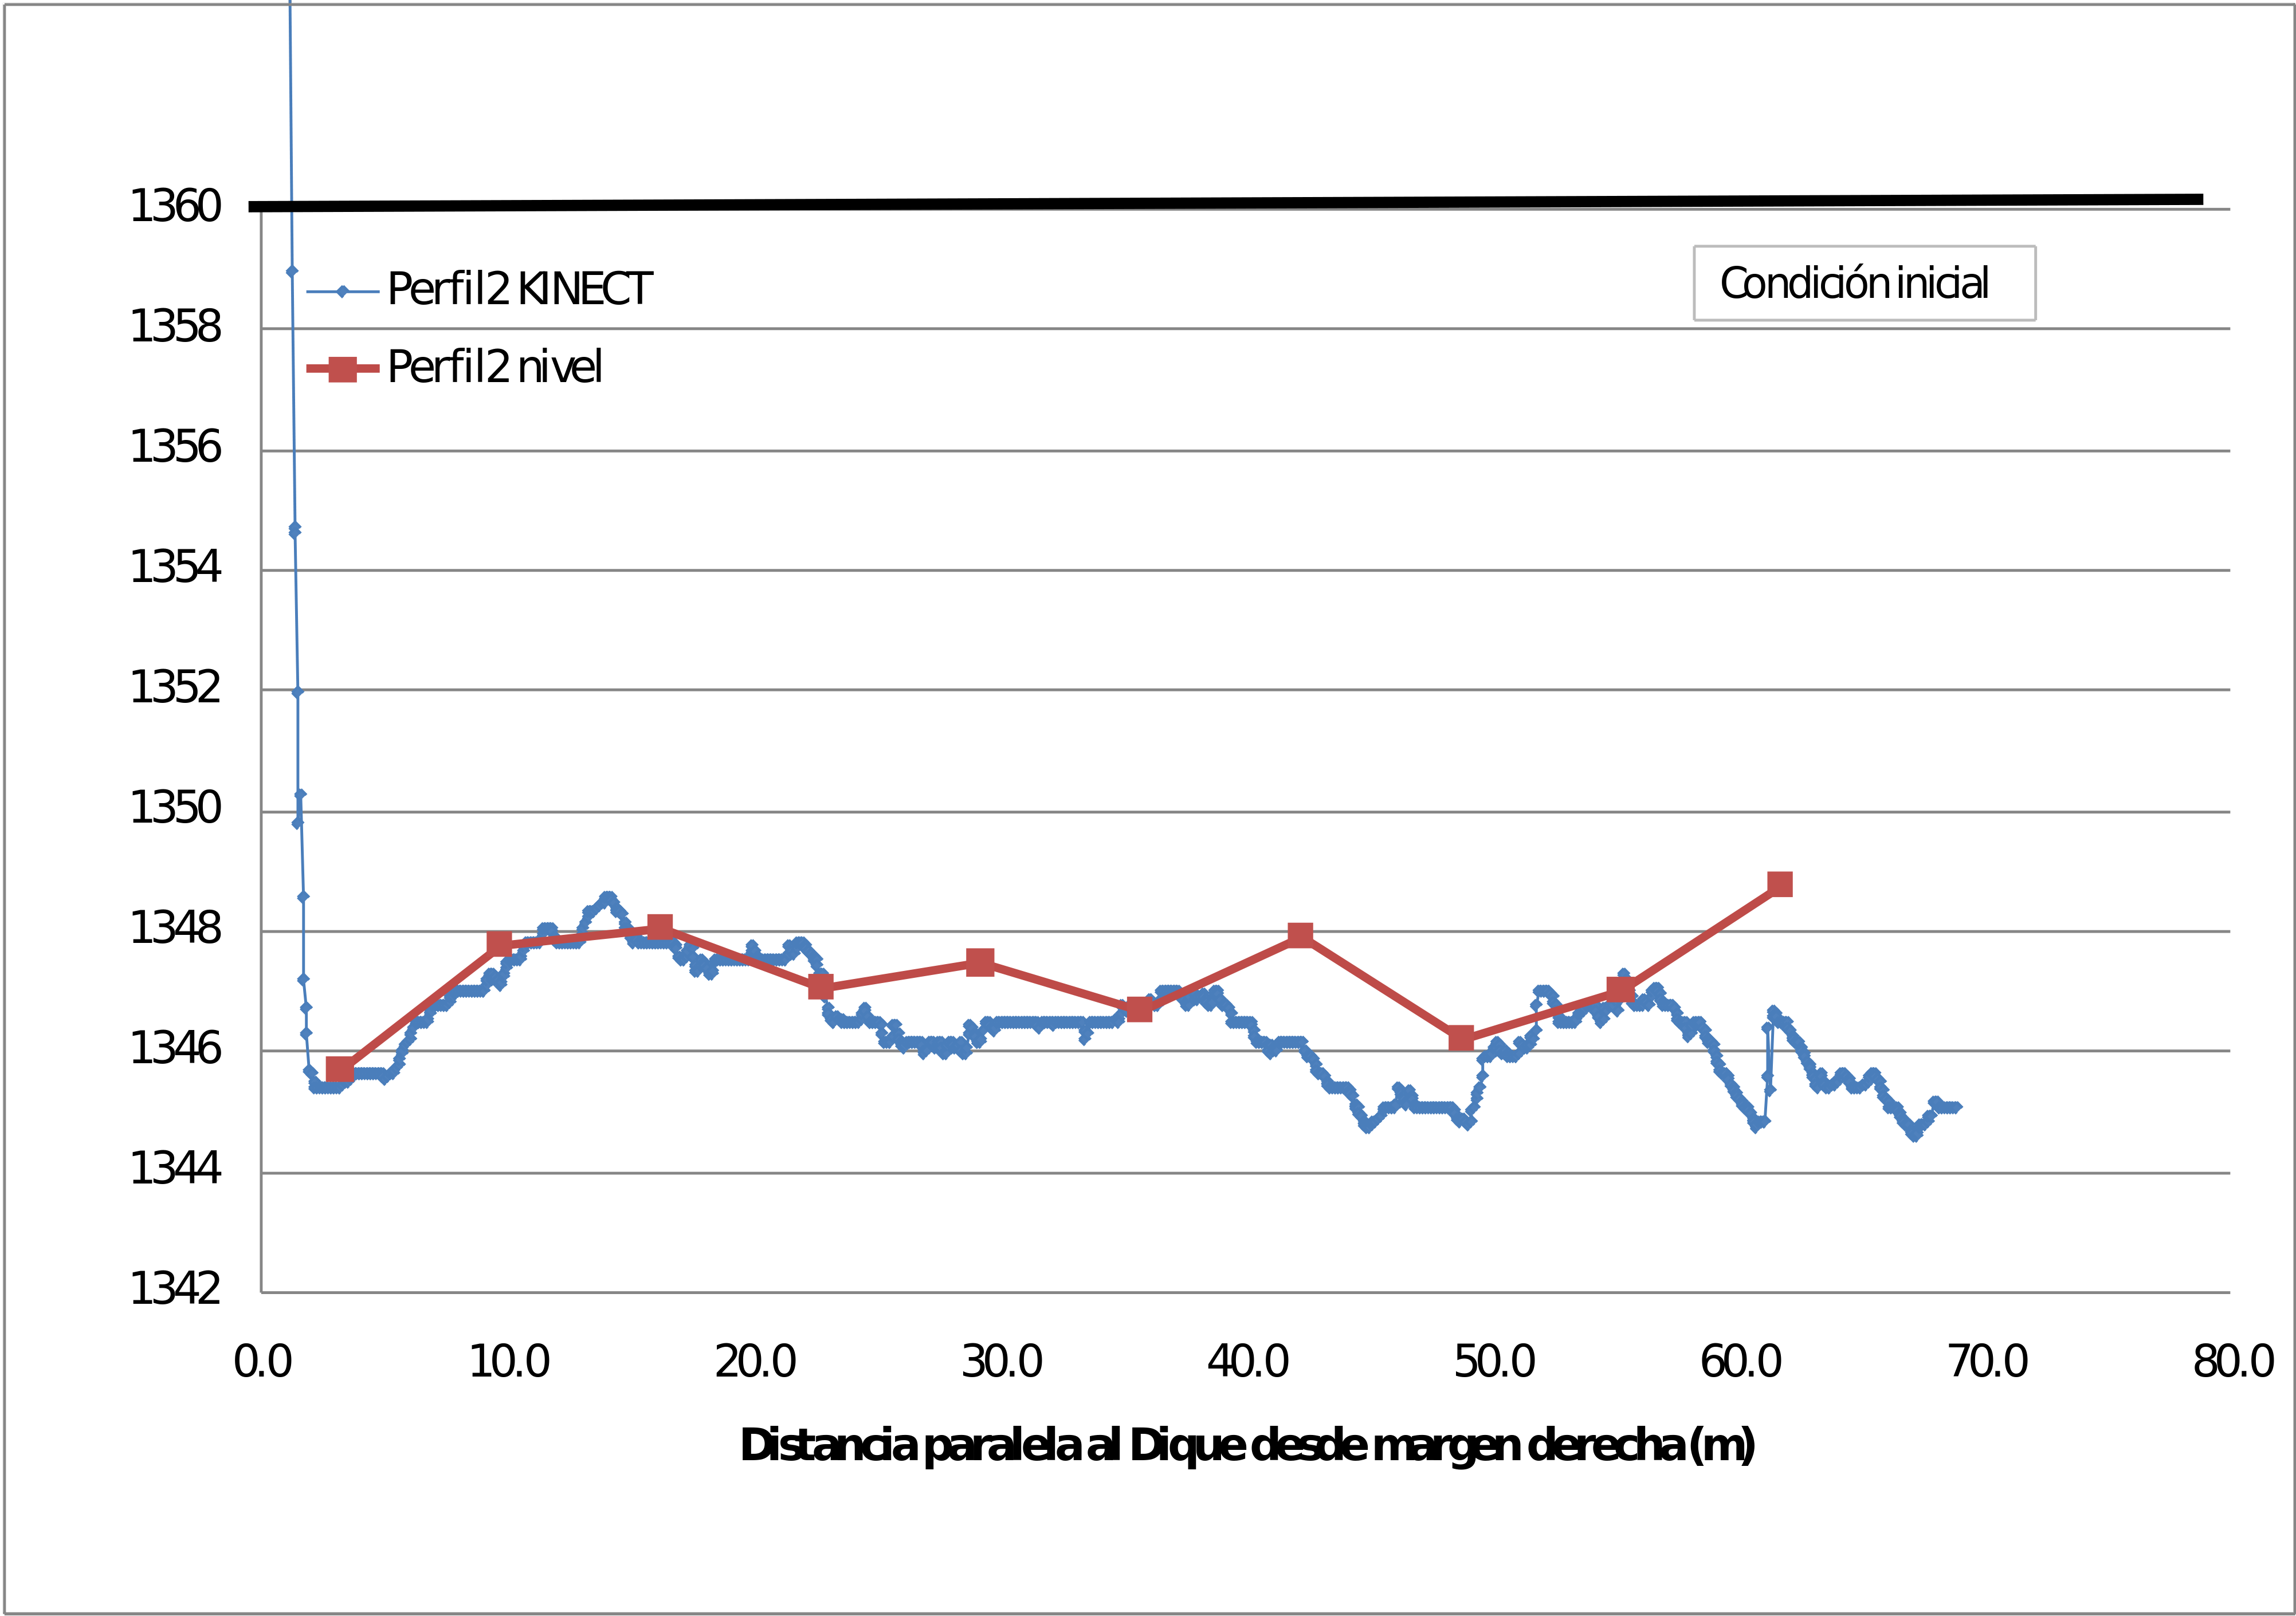
\includegraphics[width=\imsizeS]{foso-erosion-centro}
\end{center}
\end{minipage}
\hfill
\begin{minipage}[h]{.45\textwidth}
\begin{center}
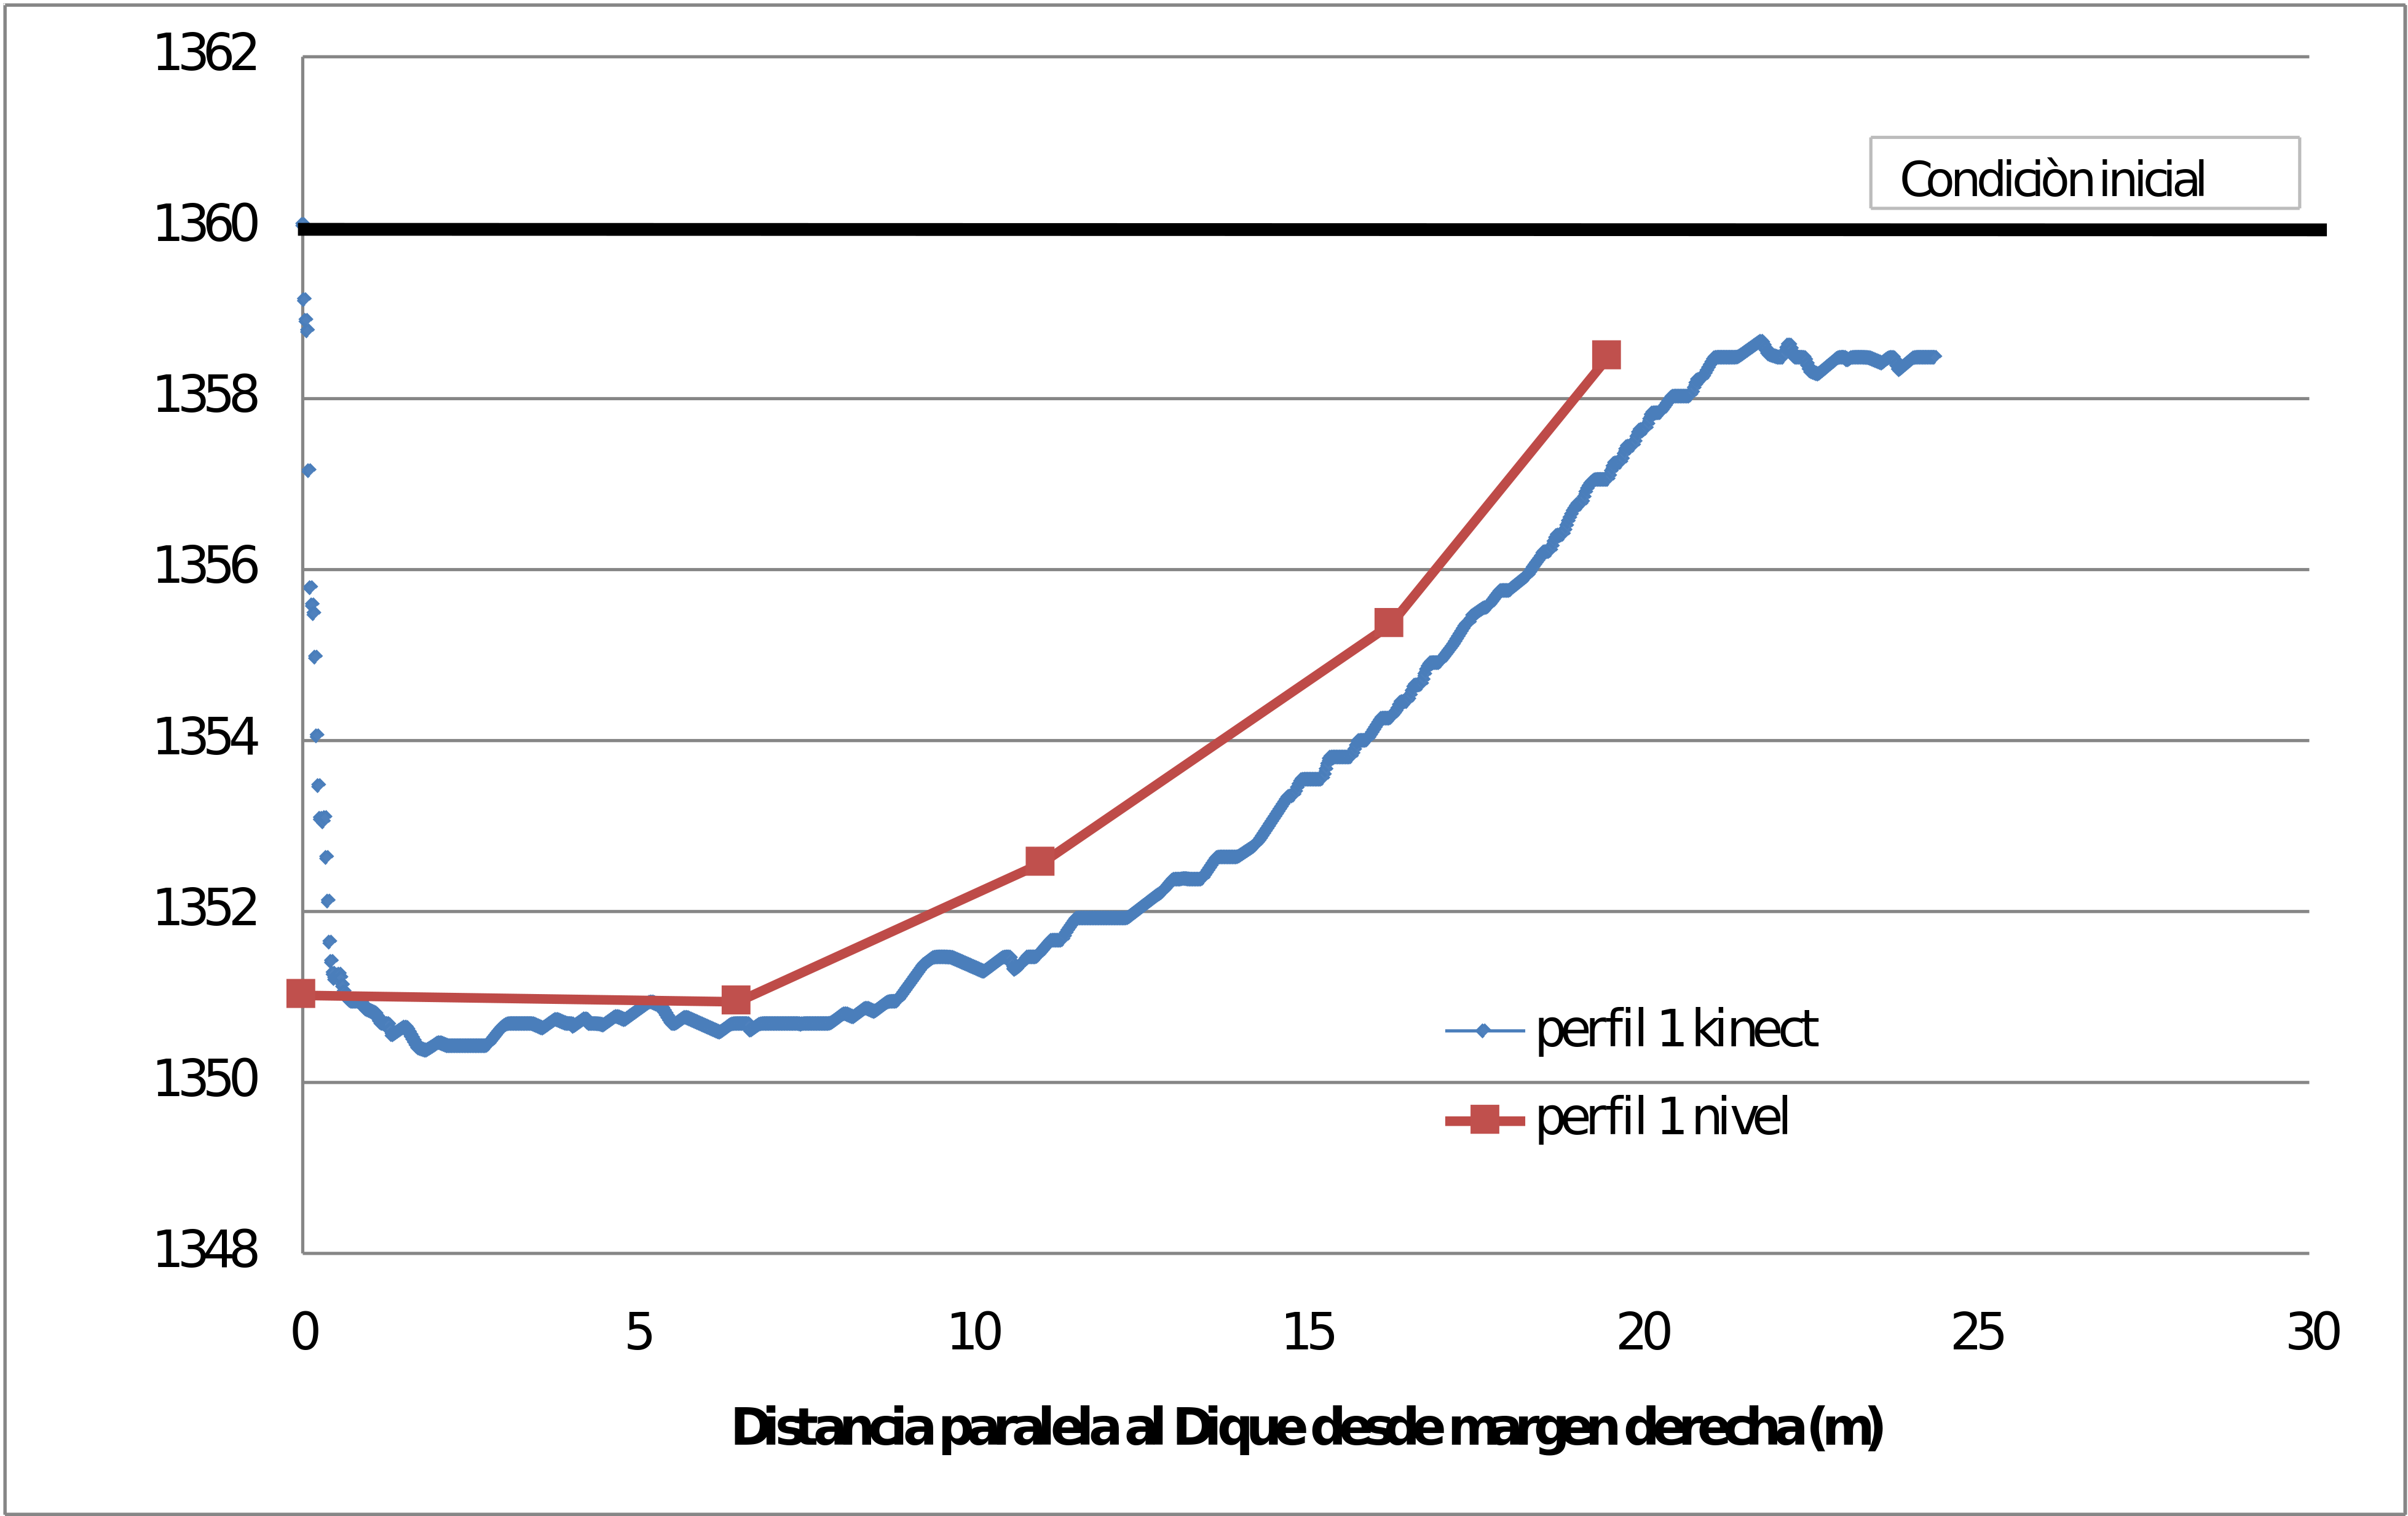
\includegraphics[width=\imsizeS]{foso-erosion-derecha}
\end{center}
\end{minipage}
\hfill
\caption[Comparación de perfiles del foso de erosión con nivel óptico y cámara Kinect]
{Comparación de perfiles del foso de erosión relevados con nivel óptico y con cámara Kinect.}
\label{fig:comparacion-perfiles}
\end{figure}

\newpage % Salto de página para acomodar las imágenes

\section{Erosión máxima}
A continuación se presentan las máximas erupciones observadas en el foso de erosión aguas abajo del canal moderador y el dique móvil relevando tanto con nivel y mira como con la cámara RGB-D.

\begin {table}[H]
\caption {Máximos niveles de erosión en el Canal Moderador} 
\label{tab:erosion-maxima-cm} 
\begin{center}

\begin{tabular}{|c|c|c|c|c|c|}
\hline 
Caudal $m^{3}/s$&Ensayo&Nivel óptico (m)&Kinect (m)&Diferencias &Diferencias\\
                &      &                &          &absolutas en &absolutas en\\
                &      &                &          &prototipo (m)&modelo (mm)\\ 
\hline 
90 & 4 & 1350.96 & 1350.37 & 0.59 & 9.07\\ 
\hline 
600 & 14 & 1349.5 & 1349.16 & 0.34 & 5.23 \\ 
\hline 
900 & 1 & 1344.8 & 1345.75 & 0.95 & 14.61\\ 
\hline 
1600 & 13 & 1345.7 & 1345.38 & \textbf{0.32} & \textbf{4.92}\\
\hline
4200 & 7 & 1345.2 & 1345.59 & 0.39 & 6\\ 
\hline 
4200 & 9 & \textbf{1344.6} & \textbf{1344.18} & 0.42 & 6.46 \\ 
\hline 
     &   &        & Promedio & 0.501 & 7.71 \\    
\hline 
     &   &        & Desv. estándar & 0.218 & 3.36 \\
\hline 
\end{tabular}
\end{center}
\end{table}

\begin {table}[H]
\caption {Máximos niveles de erosión en el Dique Móvil} 
\label{tab:erosion-maxima-dm}
\begin{center}
 
\begin{tabular}{|c|c|c|c|c|c|}
\hline 
Caudal $m^{3}/s$&Ensayo&Nivel óptico (m)&Kinect (m)&Diferencias &Diferencias\\
                &      &                &          &absolutas en &absolutas en\\
                &      &                &          &prototipo (m)&modelo (mm)\\ 
\hline 
220 & 5 & 1354.2 & 1354.89 & 0.69 & 10.61 \\ 
\hline 
600 & 14 & 1350.1 & 1349.67 & 0.43 & 6.61 \\   
\hline 
900 & 1 & 1346.1 & 1345.86 & 0.24 & 3.69 \\ 
\hline 
4200 & 7 & \textbf{1342.3} & \textbf{1343.2} & 0.9 & 13.84 \\  
\hline 
4200 & 9 & 1343.2 & 1343.41 & \textbf{0.21} & \textbf{3.23} \\
\hline 
     &   &        & Promedio & 0.493 & 7.6 \\
\hline 
     &   &        & Desv. estándar & 0.265 & 4.08 \\
\hline 
\end{tabular}
\end{center}
\end{table}

\begin{figure}[ht]
\centering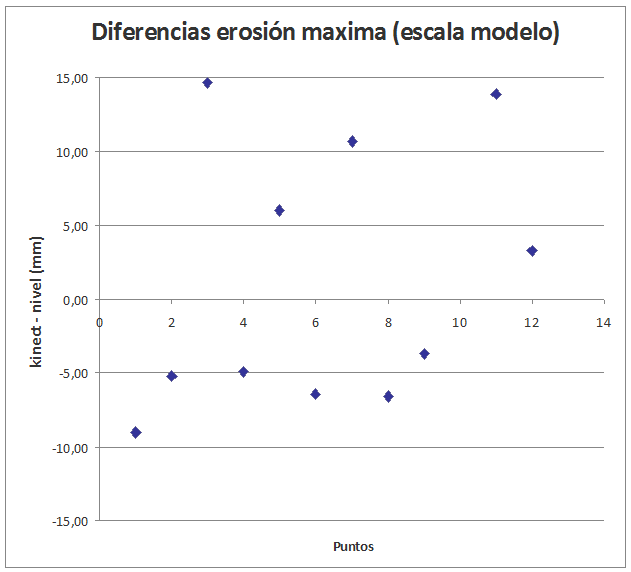
\includegraphics[width=\imsizeS]
{diferencias-erosion-maxima-modelo}
\caption[Diferencias entre mediciones de erosión máxima Kinect y Nivel]
{Diferencias (con signo) entre mediciones de erosión máxima relevadas con Kinect y con nivel óptico (en escala modelo).}
\label{fig:diferencias-erosion-maxima-modelo}
\end{figure}

Se observó un promedio en las diferencias absolutas de 7.7 mm aproximadamente y una desviación estándar de hasta 4 mm. Teniendo en cuenta que la técnica tradicional contempla errores de hasta 15 mm y el error asociado al sensor de profundidad de la Kinect es de hasta 5 mm, se considera que las mediciones realizadas con la tecnica digital estan dentro del rango aceptable para ensayos de erosión máxima. \\
Se llevó a cabo un análisis de regresión lineal simple (correlación) entre las mediciones realizadas con ambas técnicas (en escala prototipo) y se obtuvo un coeficiente de correlación $R^{2} = 0.976$, mostrando efectivamente que las mediciones entre ambas técnicas están altamente correlacionadas.

\begin{figure}[ht]
\centering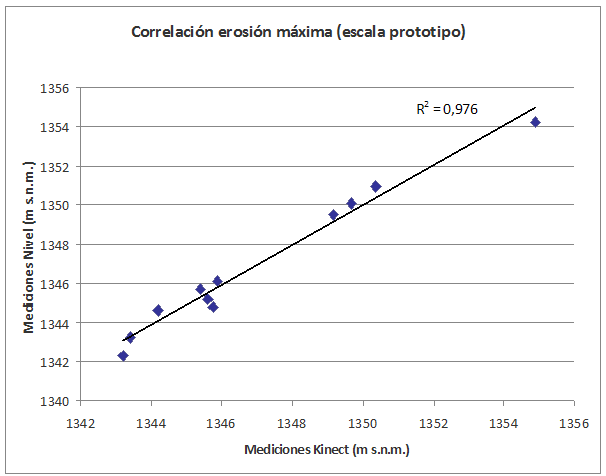
\includegraphics[width=\imsizeS]
{correlacion-erosion-maxima-prototipo}
\caption[Análisis de correlación entre mediciones de erosión máxima Kinect y Nivel]
{Análisis de correlación entre mediciones de erosión máxima Kinect y Nivel en escala prototipo. Se obtiene un $R^{2} = 0.976$.}
\label{fig:correlacion-erosion-maxima-prototipo}
\end{figure}

\section{Relevamiento de canalizaciones}

En este apartado se estudia las bondades que presenta la técnica digital para relevar el modelo físico con precisión global y se realizaron una comparación con respecto a los resultados derivados de aplicar la técnica tradicional. \\
En la sección \ref{sec:ensayo-formas-de-fondo} se presentan los resultados obtenidos para uno de los ensayos hidráulicos realizados que estudia formas de fondo generadas aguas arriba del dique para un caudal de $600 m^{3}/s$. \\
La problemática asociada a este tipo de estudios radica en la necesidad de relevar áreas extensas y con alta densidad de puntos. relevando puntos equidistantes sobre varios perfiles transversales y añadiendo la medición de puntos extras que se consideran representativos en la definición de las canalizaciones resultantes. Para obtener una aproximación global de las canalizaciones se debe generar un modelo 3D utilizando metodos de interpolacion \cite{wiki-interpolacion}.

\begin{figure}[ht]
\centering
\begin{minipage}[h]{.45\textwidth}
\begin{center}
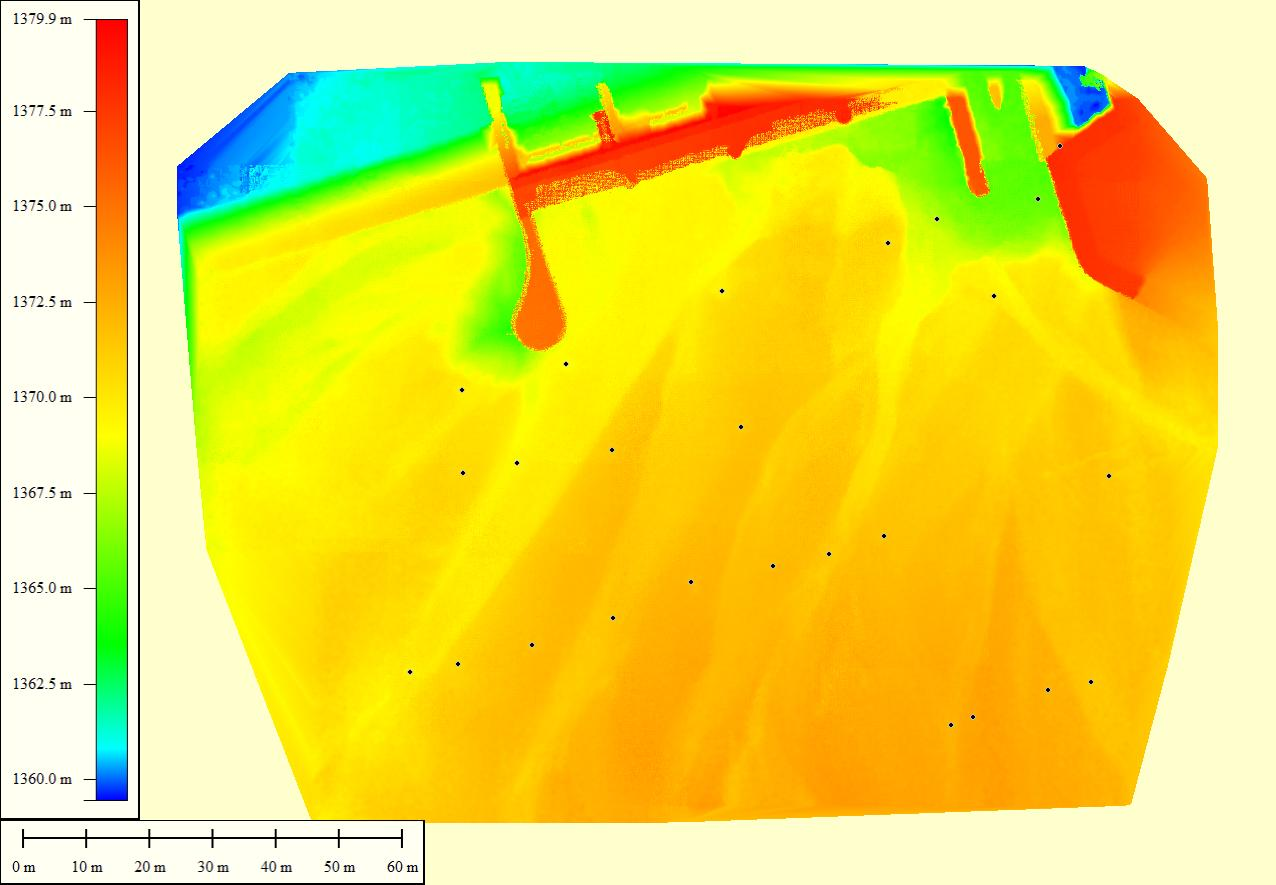
\includegraphics[width=\imsizeS]{dem-kinect}
\end{center}
\end{minipage}
\hfill
\begin{minipage}[h]{.45\textwidth}
\begin{center}
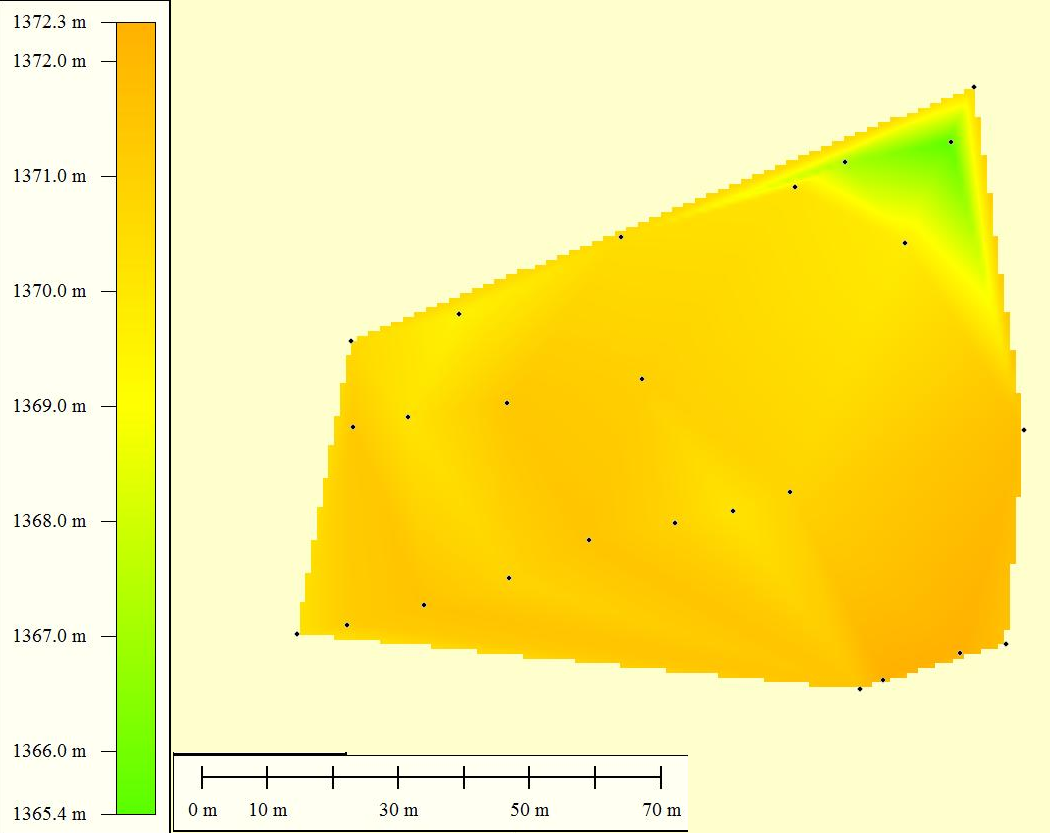
\includegraphics[width=.95\textwidth]{dem-interpolacion-nivel}
\end{center}
\end{minipage}
\hfill
\caption[DEM obtenido con Kinect y DEM generado por interpolación]
{Izquierda: DEM relevado por el sensor Kinect. Derecha: DEM generado utilizando interpolación a partir de los puntos medidos con nivel óptico. Se superponen las mediciones con nivel sobre ambos DEM's a modo ilustrativo.}
\label{fig:comparacion-dem-kinect-interpolacion}
\end{figure}

En la figura \ref{fig:comparacion-dem-kinect-interpolacion} se presentan la superficie generada por medio de interpolación a partir de puntos medidos con nivel óptico (derecha) y el modelo 3D relevado con la Kinect (izquierda) sobre la misma zona. \\
Con el objetivo de analizar la fidelidad de esta aproximacion, se trazaron un par de perfiles (sobre la misma zona), uno por cada superficie, y se calcularon las diferencias entre los resultados obtenidos con la tecnica digital y los derivados de la tecnica tradicional. En la figura \ref{fig:perfiles-diferencia-kinect-interpolacion} se presenta este experimento para cuatro cortes distintos. Se pueden apreciar zonas con diferencias de mediciones (con respecto a los valores en prototipo) dentro del intervalo $\pm0,5$ m. Este intervalo representa en modelo $\pm 7,69$ mm, lo que se considera aceptable en cuanto a la precisión de mediciones longitudinales intrusivas que se pueden alcanzar en modelos físicos. No obstante, este analisis muestra que existen dentro de estas extensas áreas relevadas, zonas donde las canalizaciones relevadas con la tecnica digital tienden a estar ubicadas entre $0,5$ m a $1,5$ m (en escala prototipo) por debajo de las canalizaciones aproximadas. Estos resultados derivan del hecho que la precision asociada a metodos de interpolacion disminuye cuando la funcion se aleja de las mediciones reales. \\
La discrepancia entre los distintos modelos 3D es demasiado alta, lo que refleja que la aproximación por interpolación no representa de forma precisa la condición real . \\
Cabe recalcar, que se puede disminuir el error presente en la superficie aproximada incrementando la cantidad de puntos relevados con la técnica tradicional (nivel y mira). Sin embargo, es simple inducir que la tecnica tradicional implica mayor tiempo de medición para relevar areas extensas con la densidad de puntos necesaria para estudios de formas de fondo. Y este proceso es tedioso cuando se deben realizar ensayos consecutivos y secuenciales asociados a aspectos complementarios del estudio global. En vista de lo anterior, se concluye que el enfoque propuesto en este trabajo permite obtener una fiel caracterizacion de las canalizaciones con un bajo costo-tiempo de medicion, resolviendo asi la problematica asociada a este tipo de ensayos. \\

\begin{figure}[ht]
\centering
\begin{minipage}[h]{.45\textwidth}
\begin{center}
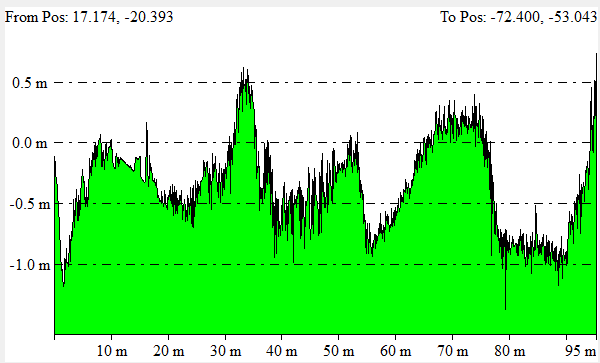
\includegraphics[width=.92\textwidth]{perfil-diferencias-kinect-interpolacion-1}
\end{center}
\end{minipage}
\hfill
\begin{minipage}[h]{.45\textwidth}
\begin{center}
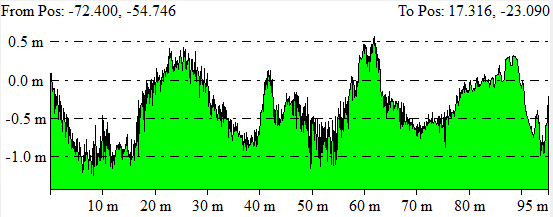
\includegraphics[width=\imsizeS]{perfil-diferencias-kinect-interpolacion-2}
\end{center}
\end{minipage}
\hfill
\begin{minipage}[h]{.45\textwidth}
\begin{center}
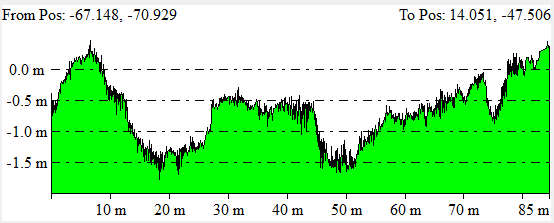
\includegraphics[width=\imsizeS]{perfil-diferencias-kinect-interpolacion-3}
\end{center}
\end{minipage}
\hfill
\begin{minipage}[h]{.45\textwidth}
\begin{center}
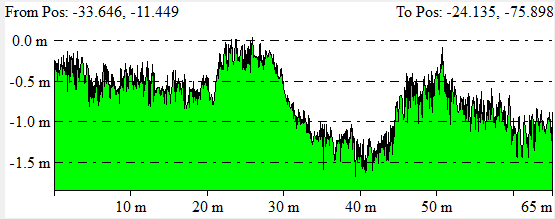
\includegraphics[width=\imsizeS]{perfil-diferencias-kinect-interpolacion-4}
\end{center}
\end{minipage}
\hfill
\caption[Diferencias entre perfiles con Kinect y perfiles extraídos desde superficie interpolada]
{Diferencias entre perfiles relevados con la técnica digital y perfiles trazados sobre una superficie interpolada a partir de mediciones con la técnica tradicional.}
\label{fig:perfiles-diferencia-kinect-interpolacion}
\end{figure}

\section{Control de estructuras del dique}

En la presente sección se analiza la precisión de la técnica propuesta para representar estructuras del dique.
En las figura \ref{fig:perfil-muro-de-encauzamiento-longitudinal}, se muestra un perfil longitudinal sobre el muro de encauzamiento. Se puede observar que la representación es precisa, conservando la forma general de la estructura, pero se advierte la presencia de algunas fluctuaciones y pequeños picos. Para analizar la magnitud del error, se trazó un perfil de menor longitud (figura \ref{fig:perfil-muro-de-encauzamiento-corto}). Se obtiene que casi todos los puntos relevados se encuentran respecto del valor 1375,1 m, el cual es la cota real de la estructura en prototipo, en el intervalo $\pm 0,3$ m (exceptuando 3 observaciones a 0,35 m, 0,4 m, 0,45 m respectivamente). Esto indica que una diferencia de 0,3 m en prototipo o equivalentemente 4.61 mm en modelo, condición que se mantiene dentro del margen esperado de 5 mm, posicionando la cámara a una distancia menor a 1,5 m (apartado \ref{sec:consideraciones-kinect}). En la figura \ref{fig:perfil-muro-de-separacion}, se traza un perfil longitudinal sobre el muro de separación del dique fijo y el canal moderador, y se obtienen valores en el intervalo 1376,27 m $\pm 0,25$ m, es decir, un error aproximado de 3,84 mm en modelo, similar a lo observado anteriormente. \\
En la figura \ref{fig:perfil-muro-de-encauzamiento-longitudinal} destacan 2 observaciones aisladas con error de aproximadamente 6 cm en escala modelo que no pudieron ser filtradas. Se propone continuar en trabajos futuros el estudio de una metodología eficaz para eliminar este tipo de \textit{outliers}. \\
Se concluye que la técnica propuesta captura con precisión aceptable las estructuras del dique, lo que habilita a poder utilizar dichas estructuras como referencias visuales en el estudio de la erosión.

\begin{figure}[ht]
\centering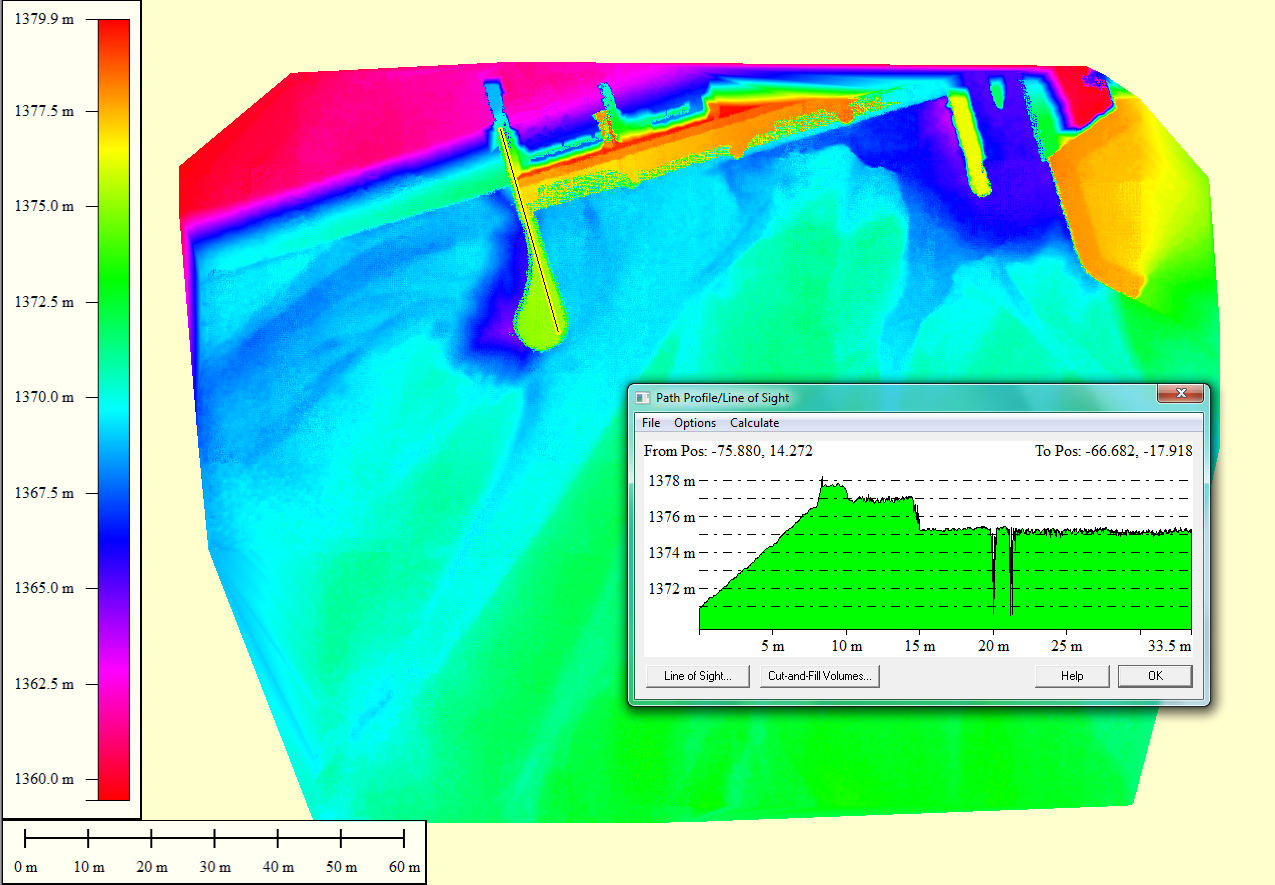
\includegraphics[width=\imsize]
{perfil-muro-de-encauzamiento-longitudinal}
\caption[Perfil longitudinal sobre el muro de encauzamiento]
{Perfil longitudinal sobre el muro de encauzamiento.}
\label{fig:perfil-muro-de-encauzamiento-longitudinal}
\end{figure}

\begin{figure}[ht]
\centering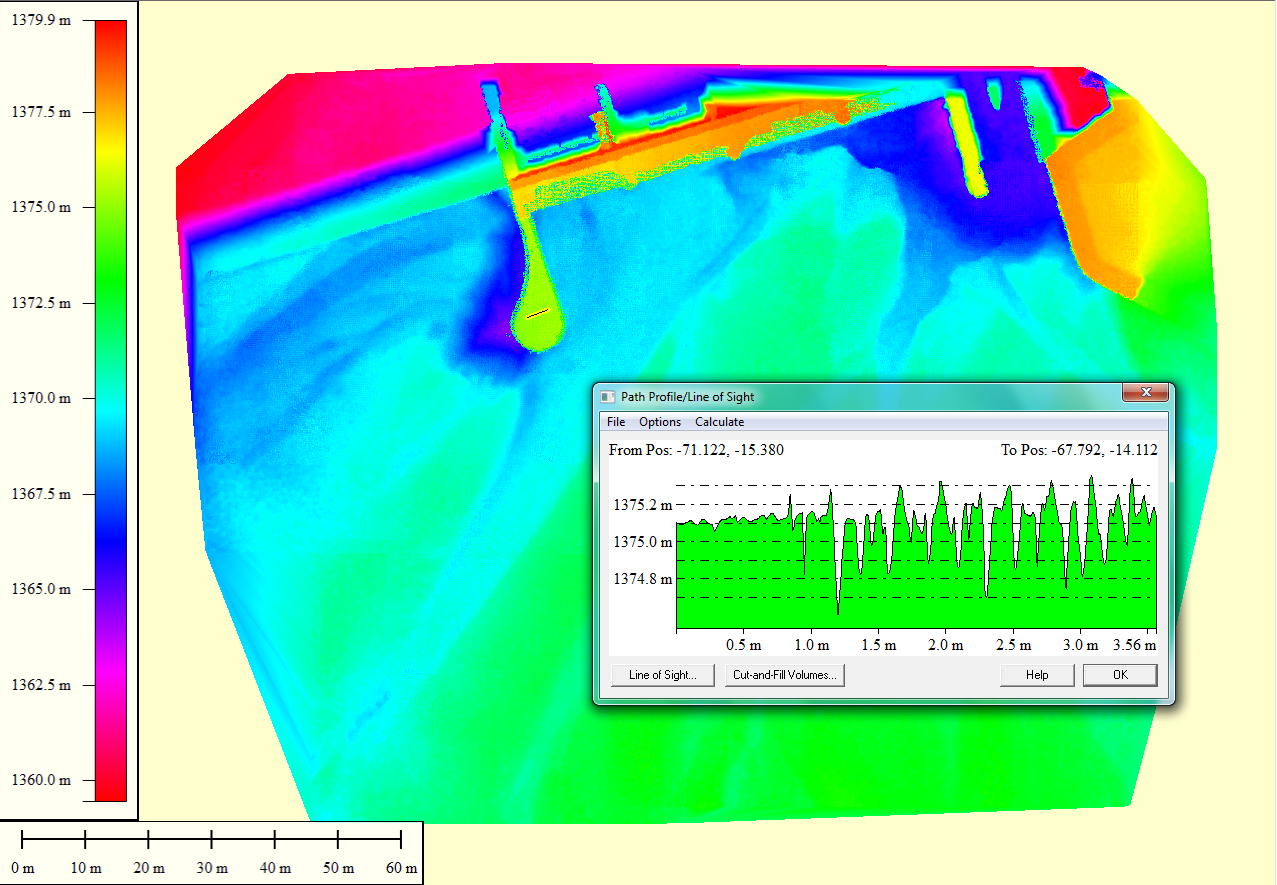
\includegraphics[width=\imsize]
{perfil-muro-de-encauzamiento-corto}
\caption[Perfil corto sobre el muro de encauzamiento]
{Perfil corto sobre el muro de encauzamiento.}
\label{fig:perfil-muro-de-encauzamiento-corto}
\end{figure}

\begin{figure}[t]
\centering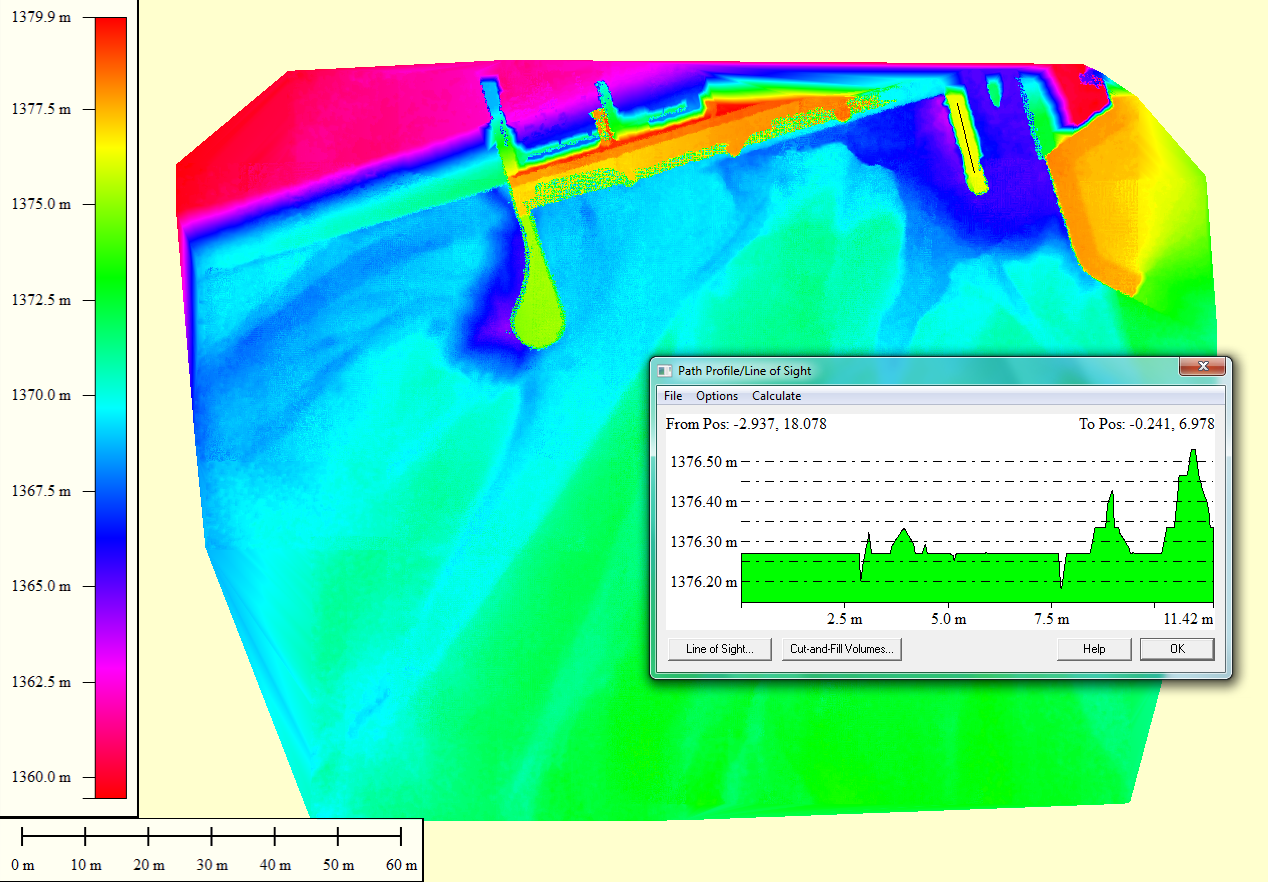
\includegraphics[width=\imsize]
{perfil-muro-de-separacion}
\caption[Perfil sobre el muro de separación entre el dique móvil y el canal moderador]
{Perfil sobre el muro de separación entre el dique móvil y el canal moderador.}
\label{fig:perfil-muro-de-separacion}
\end{figure}




\begin{biblio}
\bibliography{mibib}
\end{biblio}

\begin{postliminary}

\begin{seccion}{Publicaciones asociadas}
  \begin{enumerate}

  \item SIMPOSIO DE METODOS EXPERIMENTALES EN HIDRAULICA, SANTA FE, \textbf{2013}

  \item XXIV CONGRESO NACIONAL DEL AGUA, SAN JUAN, \textbf{2013}

  \end{enumerate}
\end{seccion}

%\begin{seccion}{Agradecimientos}
%A todos los que se lo merecen, por merecerlo
%\end{seccion}

\end{postliminary}

\end{document}